\documentclass[../main.tex]{subfiles}

\begin{document}

\renewcommand{\labelitemi}{\ding{226}}
\renewcommand{\labelitemii}{\ding{227}}


\part{Introduction}
\label{part:intro:general}

\chapter{Neutrino physics}
\label{ch:nu_phys}
Exploration of the neutrinos is a very promising direction of research in particle physics. Over the last 60 years since its first experimental observation, several breakthroughs were made. Many of them have been awarded notable prizes. All this speaks of the great interest of the community on this topic. Many puzzles are still unsolved, several challenging experiments are ongoing.

Neutrino was always a kind of ``mysterious'' particle. It was proposed as an almost undetectable particle to explain the unexpected behavior of the beta decay (\autoref{sec:hist}). It remained a hypothesis for 36 years until it was finally observed in the breakthrough experiment. After the first detection, a new puzzle was found. The neutrino flux from the Sun was much lower than expected. Both Solar and neutrino models remained in doubt for 40 years until the phenomenon of the missing neutrinos was solved. It led to the discovery of an extremely interesting effect --- neutrino oscillations (\autoref{sec:intro:osc}). It was found that neutrinos are changing flavor while propagating in the vacuum. This fact indicates that neutrino has non-zero masses, as only massive particles can change their state in time.

The non-zero neutrino mass triggered several hypotheses about its origin (\autoref{ch:intro:HNL}). It can't be explained within the Standard Model --- the main framework in particle physics. Hence this fact can indicate a new unexplored region of fundamental physics. One of the most probable explanation is the existence of the new particle(s). Such a hypothesis can have many applications, such as the explanation of the Dark Matter phenomenon. Thus the explorations in the neutrino physics can lead to very interesting discoveries.

Another interesting subject is a charge--parity violation in the neutrino oscillations (\autoref{sec:intro:cp}). Some hints were found that the neutrino oscillation process is not symmetric under the change of particle charge and the space inversion. This effect together with the existence of the new particles can explain the phenomenon of the matter-dominance in the Universe (\autoref{sec:intro:numsm}).

To sum up, neutrino physics is a very promising field of research with several open challenges and interesting results awaiting.

\section{Historical overview}
\label{sec:hist}
The prerequisites of the neutrino existence were found at the beginning of the XXth century. The spectrum of the electrons from the $\beta$-decay was measured to be continuous~\cite{Chadwick1914}. The $\beta$-decay corresponds to a neutron transformation into electron and proton. Following the laws of both momentum and energy conservation, the electron produced in the 2-body decay should have fixed energy defined by the mass difference between the neutron and the proton. Non-discrete spectrum provoked several theories such as energy non-conservation (by N. Bohr) or existence of the new hypothetical particle (by W. Pauli~\cite{Pauli1930}). Later Enrico Fermi developed a complete theory of beta decay~\cite{Fermi1934}. In the modern notation, the decay process was presented as $n\to p^++e^-+\overline{\nu}_e$, where neutrino is noted as $\nu$.

\subsection{Discovery of the neutrino}
The experimental discovery of the neutrino was quite challenging. Neutrinos are not taking part in the electromagnetic or strong interactions. The only way to detect them is through the weak interaction. Based on Fermi's theory, along with the beta decay $n\to p+e^-+\overline{\nu}_e$ the inverse beta decay $\overline{\nu}+p\to n+e^+$ should exist. Such a process can be used for the direct detection of the neutrino. But the expected cross-section for such a process was estimated to be at the level of $10^{-44} \text{ cm}^2$. That was about a couple of dozen orders of magnitude less than cross-sections of other known processes. That's why the neutrino discovery happened only 26 years after the idea of the neutrino existence had been proposed.

After the proposal of the new particle few indirect measurements were performed, but the direct observation remained a challenge. The first successful neutrino detection was done by the group led by Frederick Reines and Clyde Cowan~\cite{Cowan1956}. They performed a series of experiments trying to detect neutrino from the most powerful source at that time - nuclear power plant. Relatively new material a liquid scintillator was used as a target and detector. The inverse beta decay was used as a detection reaction:
\begin{equation}
\bar{\nu}+p\to n+e^+
\end{equation}
The positron shortly annihilates emitting two photons that can be detected with photomultipliers (PMTs). But not only neutrino interactions can cause such a signal. To suppress the background, a Cadmium isotope was added to the detector. Thus the neutrons would also be detected with reaction
\begin{equation}
n+{}^{108}Cd\to{}^{109m}Cd\to{}^{109}Cd+\gamma
\end{equation}
As the ${}^{109m}Cd$ lifetime is few tens of microseconds the signal will have a unique signature: positron annihilation, followed by the gamma-ray emission with a known delay time. Thus rare signal events can be separated from a variety of backgrounds.

Such a strategy lead to the successful discovery of the particle that was supposed to be ``undetectable'' before.

\subsection{Neutrino flavors}
\label{sec:dublet}
The first neutrino detection was made using a nuclear reactor as a particle source. Such a source is extremely powerful but isotropic. For the precise measurements, it will be extremely useful to gain the statistics with the focused particle beam. For this, accelerators can be used. The general idea is to use a proton beam hitting a target to produce mesons. The charged meson can be focused with a magnetic field and further decay, producing the focused neutrino beam with high intensity. The description of such a scheme in the modern experiment can be found in \autoref{ch:T2K:nu_beam}. This approach was used the first time to determine if the neutrino has flavors~\cite{Danby1962}. At that time it was known that there are two generations of the charged leptons: electron and muon. The question was if the electron neutrino was different from the muon neutrino. The main idea of the experiment is to use the neutrino flux produced from the pion decay. Because of the mass difference between electron and muon charged pion decays mainly to the muon, e.g. $\pi^+\to\mu^++\nu_\mu$. The experiment showed clearly that the reaction \autoref{eq:notallowed} is severely suppressed comparing the reaction \autoref{eq:allowed}.

\begin{align}
\label{eq:allowed}
\nu_\mu+p&\rightarrow n+\mu \\
\nu_\mu+p&\nrightarrow n+e
\label{eq:notallowed}
\end{align}

That means that neutrino has flavors. It can be either produced or detected with the lepton of the same flavor. The existence of the different types of neutrino confirmed the doublet structure of the leptons. This fact will play an important role in the theory of neutrino oscillations (\autoref{sec:intro:osc}).

\subsection{Neutrino in the Standard Model}
\label{sec:sm}

Physicists have used gauge (``scale'') symmetries to build the field theories. It is a powerful and elegant tool. The group theory appeared to be a natural mathematical framework for the description of gauge fields. After the development of quantum mechanics, the scale was turned to a complex value. Thus the quantum electrodynamic theory was created using $U(1)$ abelian gauge group.

The first step towards the general model of particle physics was done by Yang and Mills by extending the concept of the gauge theory to the non-abelian groups $SU(2)$. This made possible to describe the phenomenon of strong interactions~\cite{Yang1954}. Later Glashow found a way to unify the electromagnetic and weak interactions~\cite{Glashow1961}. Salam and Weinberg finished the theory with the implementation of the Higgs mechanism into the Glashow theory~\cite{Weinberg1967}.

Many experiments brilliantly confirmed the proposed model and demonstrated its predictive power. For example, in the sector of the electroweak interactions, the most important observations were: neutral current discovery~\cite{Cundy1974}, the Z and W boson discovery~\cite{Arnison1983}, the $\gamma-Z$ interference, neutrino generation number~\cite{Arnison1983}, Higgs boson discovery~\cite{Aad2012}, and many others.

% The schema describing the Standard Model is presented in \autoref{fig:intro:SM}.

% \begin{figure}[!ht]
%     \centering
%     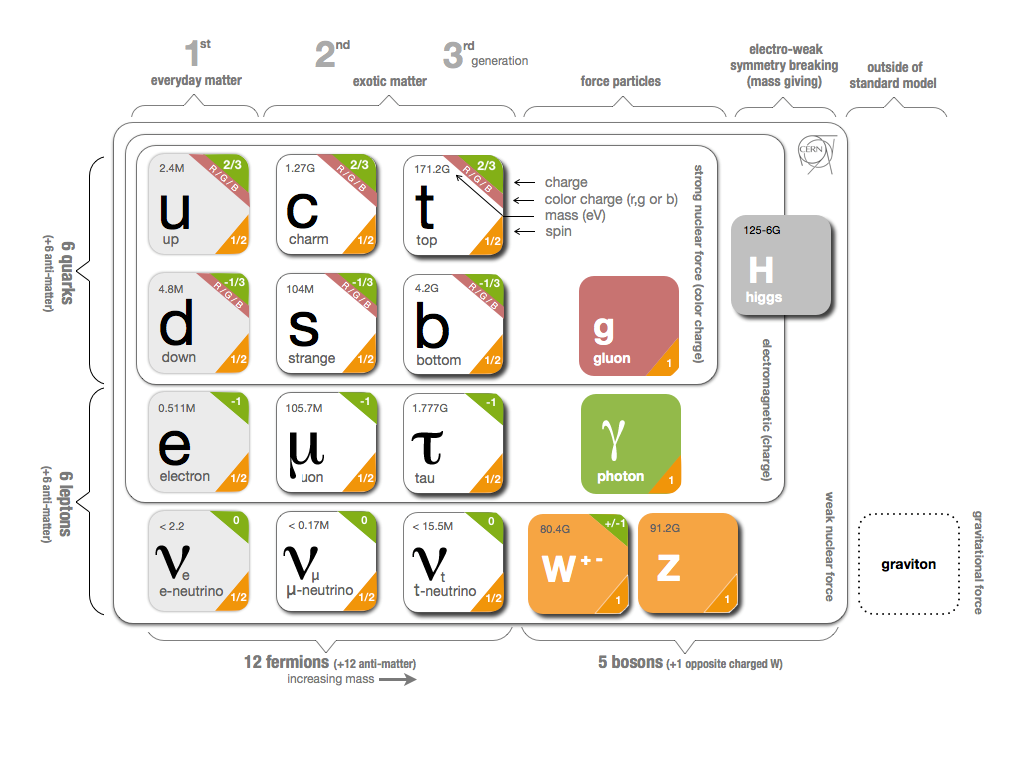
\includegraphics[width=0.8\linewidth]{SM.png}
%     \caption{A schematic view of the Standard Model (SM) of particle physics.}
%     \label{fig:intro:SM}
% \end{figure}

In general, the SM is based on the Yang--Mills theory with local $SU(3)\times SU(2)\times U(1)$ gauge symmetry. It can be divided into several sections:
\begin{itemize}
  \item Quantum chromodynamics sector
  \item Electroweak sector
  \item Higgs sector
  \item Yukawa sector
\end{itemize}

In the context of the current thesis, we will discuss in detail the electroweak sector. It is based on group $U(1)\times SU(2)_L$. It means that we will have two sets of generators: the weak hypercharge $Y_W$ for $U(1)$ and Pauli matrices for $SU(2)_L$. Index $L$ means that it affects only left-chiral fermions.

\begin{bclogo}[couleur=blue!2, arrondi=0.1, logo=\bcinfo, nobreak=true]{Helicity, polarity, chirality}
Helicity is a projection of the spin onto the direction of the momentum.
\begin{equation}
h=\frac{\vec{s}\cdot\vec{p}}{\left|\vec{s}\right|\left|\vec{p}\right|}
\end{equation}

The helicity can be ``left'' or ``right'' that corresponds to the spin direction opposite or co-directed with momentum. For the massless particles, helicity is Lorentz invariant. The polarization of the particle beam is the fraction of the particles with a given helicity. For example, 50\% polarization means that half of the particles are ``left'' and half are ``right''.

The chirality is a more fundamental characteristic compared to helicity. It is determined by whether the particle wave function transforms with a right- or left-handed representation of the Poincare group.

%Massless fermions keep chiral symmetry, i.e.
Chirality is a conserved quantum number for massless fermions. It means that independent rotation of the left- and right- handed components doesn't affect the theory. For them, the helicity is always the same as chirality.

The massive particles break the chiral symmetry explicitly. Also for the massive fermions, the helicity is not equivalent to the chirality as one can choose the reference frame moving faster than the particle and inverse the helicity.
\end{bclogo}

In the SM fermions are described as doublets (\autoref{sec:dublet}). For each charged lepton there is a corresponding neutrino. While charged lepton can be either right-handed or left-handed, the neutrino can be only left-handed. This part of the theory is based on the empirical observations~\cite{Goldhaber1958} and this is strictly fixed in the model. A neutrino can interact via the charge current (CC) or neutral current (NC). The corresponding interaction terms are written as:

\begin{align}
-\mathcal{L}_{CC}&=\frac{g}{2}\sum_\alpha\bar{\nu}_{L\alpha}\gamma^\mu\ell_{L\alpha}W^+_\mu+h.c. \\ \nonumber
-\mathcal{L}_{NC}&=\frac{g}{\sqrt{2\cos{\theta_W}}}\sum_\alpha\bar{\nu}_{L\alpha}\gamma^\mu\nu_{L\alpha}Z^0_\mu
\end{align}

Thus there is no possibility for the production or detection of the right-handed neutrino (left-handed anti-neutrino). The existence of such ``exotic'' particles is proposed in the various theories (\autoref{sec:intro:HNL}).

\subsubsection{Number of neutrino flavors}
\label{sec:intro:LEP}
After the magnificent confirmation of the Standard Model with the discovery of the neutral current and W and Z bosons, it became possible to measure precisely the number of the neutrino generations. This analysis became possible with the massive production of the Z-bosons at Large Electron-Positron Collider (LEP) at CERN.

The general idea of the study is to look at the different modes of the Z decays. These decays can be classified into several groups:

\begin{align}
Z&\to q\overline{q} \nonumber \\
Z&\to \ell^+\ell^- \\
Z&\to \nu\bar{\nu} \nonumber
\end{align}

The total width of the boson decay is a sum of these three channels. As the width of $Z\to \ell^+\ell^-$ is the same of all charged leptons and $Z\to \nu\bar{\nu}$ is the same for all neutrino types because of the lepton universality. The total $Z^0$ width can be written with:

\begin{equation}
\Gamma_Z=\Gamma(Z\to hadrons)+N_{\ell}\times\Gamma(Z\to \ell^+\ell^-) + N_{\nu}\times\Gamma(Z\to \nu\bar{\nu})
\label{eq:intro:nnu}
\end{equation}

In the experiment, $\Gamma_Z$, $\Gamma(Z\to q\overline{q})$ and $\Gamma(Z\to \ell^+\ell^-)$ were measured. The equality of the $\Gamma(Z\to e^+e^-)$ and $\Gamma(Z\to \mu^+\mu^-)$ was checked. The width of the decay into neutrinos came from the theory. The number of neutrino generations remained the only unknown variable in the \autoref{eq:intro:nnu}. The results of the precise measurements of the Z-boson resonance and predictions for 2, 3 and 4 neutrino generations are shown in \autoref{fig:intro:NuGen}. At LEP, the number of neutrino generations was measured to be $N_{\nu}=2.9840\pm0.0082$~\cite{Bagger2006}. So we can conclude that in Standard Model there are only three types of the left-handed neutrino with masses less than half of the Z-boson mass.

\begin{figure}[!ht]
    \centering
    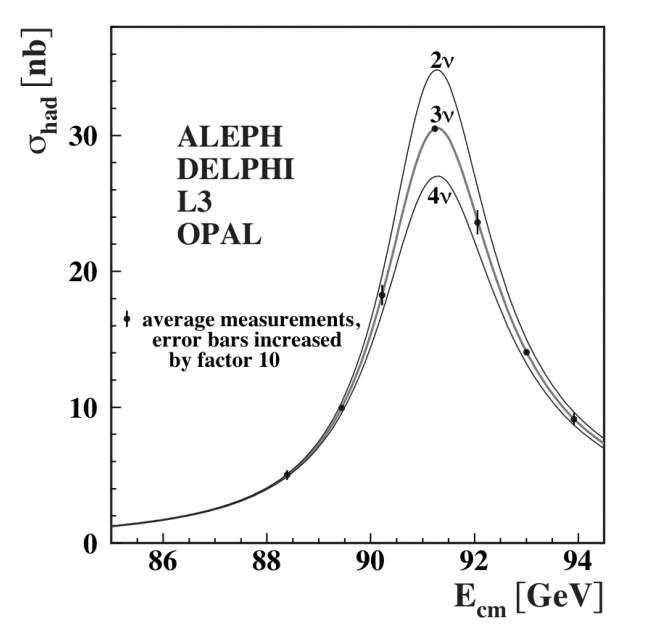
\includegraphics[width=0.6\linewidth]{Neutrino_gen.png}
    \caption{Measurement of the hadron production cross-section as a function of the LEP center-of-mass energy around the Z-boson resonance.}
    \label{fig:intro:NuGen}
\end{figure}

\section{Neutrino interactions}
The precise measurements in neutrino physics such as neutrino oscillation and search for CP--violation require accurate knowledge about the neutrino interactions' rates. This is still one of the dominating uncertainties in the experiments. Roughly we can divide the neutrino interactions with the matter on the interactions with electron and nucleus. The neutrino interactions with the single fermion are described very accurately with the Standard Model. So far no deviations are found in the experiment.

\subsection{Interactions with electron}
Neutrino interactions with the single electron are the simplest ones. They can be described with the tree-level Feynman diagrams presented in \autoref{fig:intro:f_nu}. Electron neutrino can interact with the electron both through the scattering through the charged current (\autoref{fig:intro:f_nu} (a)) and neutral current (\autoref{fig:intro:f_nu} (c)), while muon and tau neutrino can scatter\footnote{Here ``scattering'' means that the initial electron is not changing the flavor, e.g. does not transform into muon} only via neutral current.

The muon neutrino can also interact with the electron through the charged current (\autoref{fig:intro:f_nu} (b)), but this is a threshold process. The minimal neutrino energy can be estimated by $E_\nu^{th}=\left(m_\mu^2-m_e^2\right)/\left(2m_e\right)=10.9GeV$ neglecting the neutrino mass. Thus the muon can not be produced by the neutrinos from the Sun or other low-energy neutrinos.

\begin{figure}[!ht]
\centering
  \begin{minipage}[t]{0.29\linewidth}
    \centering
    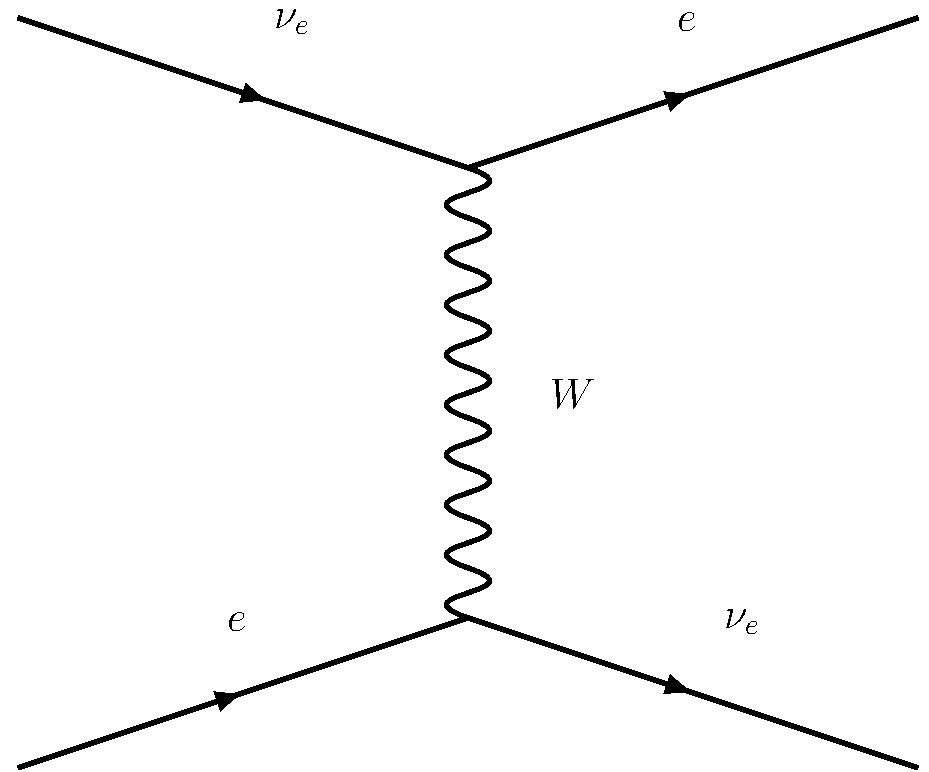
\includegraphics[width=0.8\linewidth]{fa_nue} \\ (a)
  \end{minipage}
  \begin{minipage}[t]{0.29\linewidth}
    \centering
    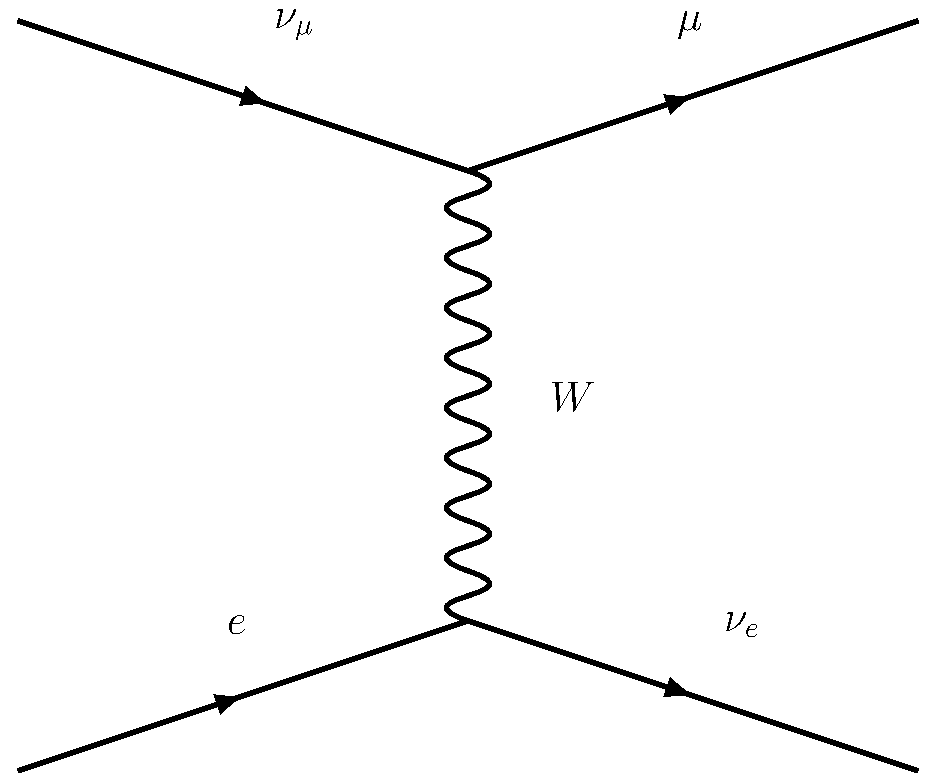
\includegraphics[width=0.8\linewidth]{fa_numu} \\ (b)
  \end{minipage}
  \begin{minipage}[t]{0.29\linewidth}
    \centering
    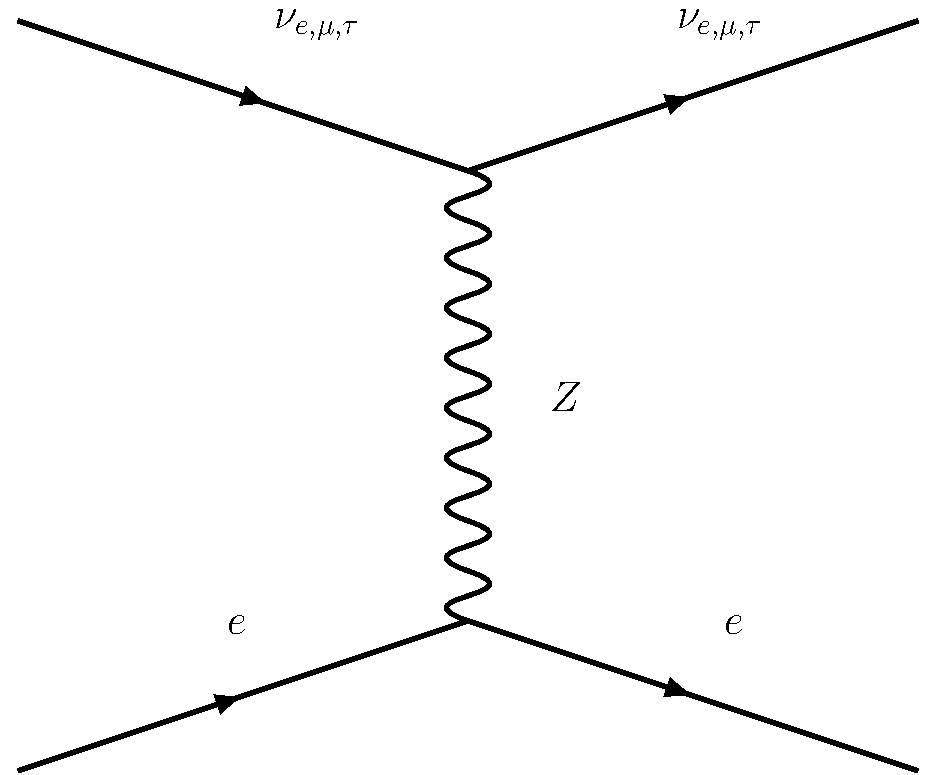
\includegraphics[width=0.8\linewidth]{fa_nu_NC} \\ (c)
  \end{minipage}
  \caption{Tree-level Feynman diagrams of the neutrino interactions with electron: (a) and (b) electron and muon neutrino scattering through the charged current, (c) all-type neutrino scattering through the neutral current.}
  \label{fig:intro:f_nu}
\end{figure}

The anti-neutrino interaction with the electron can be described with the Feynman diagrams presented in \autoref{fig:intro:f_anu}. Comparing with the neutrino case, a muon anti-neutrino can not interact with the electron through the charged current $\overline{\nu}_\mu+ e^-\nrightarrow \mu^-+\overline{\nu}_e$.

\begin{figure}[!ht]
\centering
  \begin{minipage}[t]{0.29\linewidth}
    \centering
    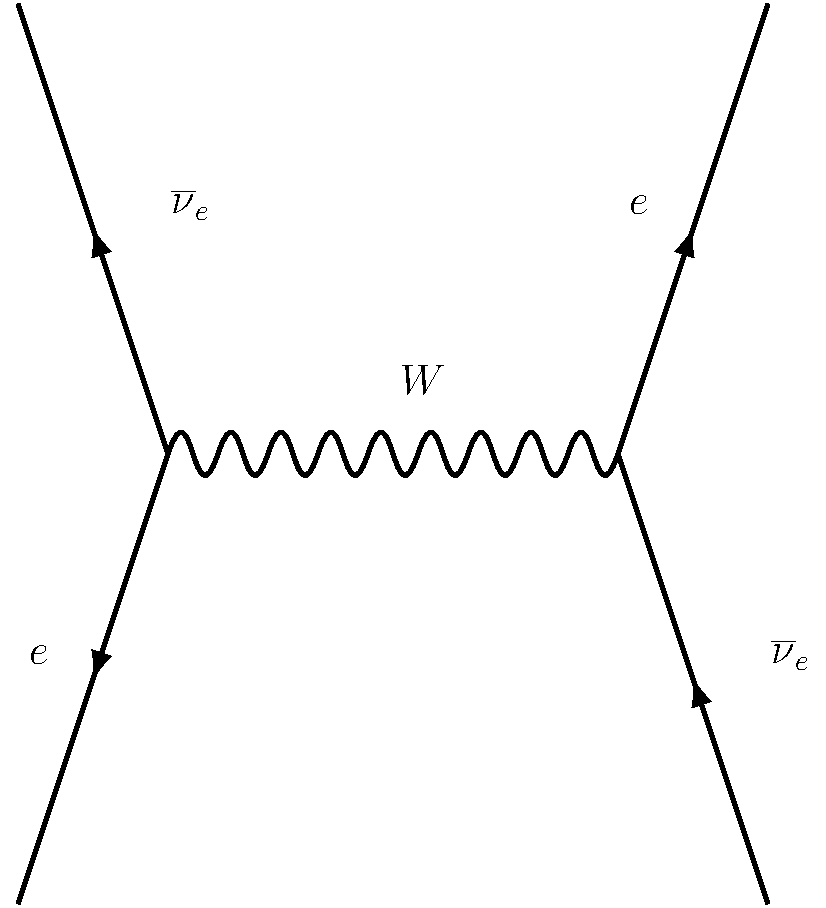
\includegraphics[width=0.8\linewidth]{fa_anue} \\ (a)
  \end{minipage}
  \begin{minipage}[t]{0.29\linewidth}
    \centering
    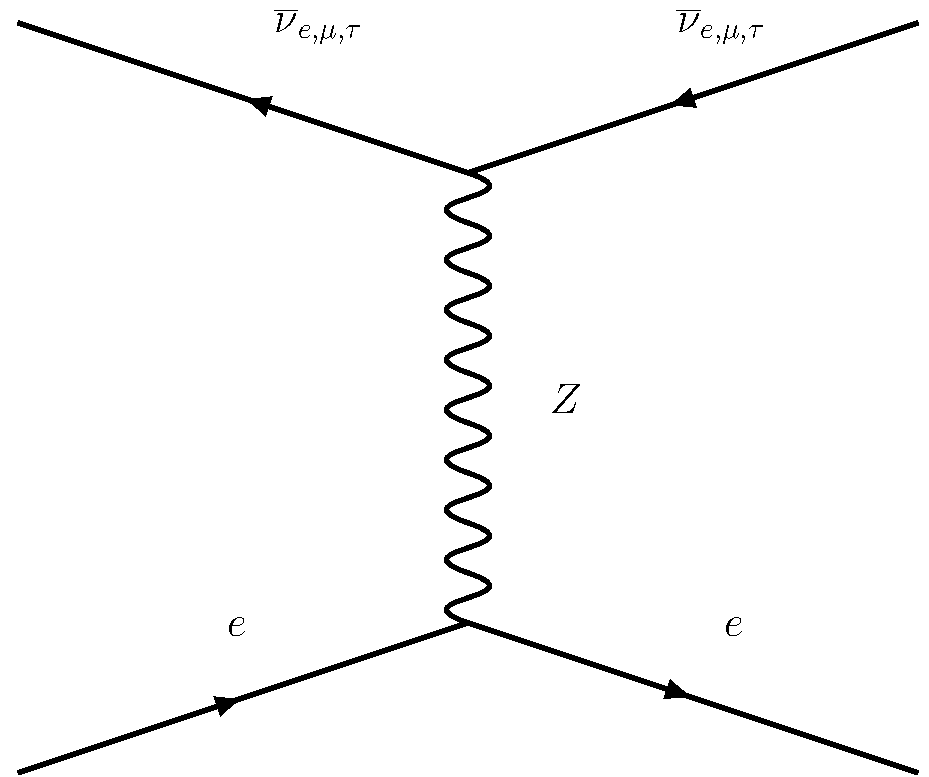
\includegraphics[width=0.8\linewidth]{fa_anu_NC} \\ (b)
    \end{minipage}
  \caption{Tree-level Feynman diagrams of the anti-neutrino interactions with electron: (a) electron anti-neutrino scattering through the charged current, (c) all-type anti-neutrino scattering through the neutral current.}
  \label{fig:intro:f_anu}
\end{figure}

The cross-sections for the processes mentioned above are presented on the \autoref{fig:intro:nue_xsec}.

\begin{figure}[!ht]
  \centering
  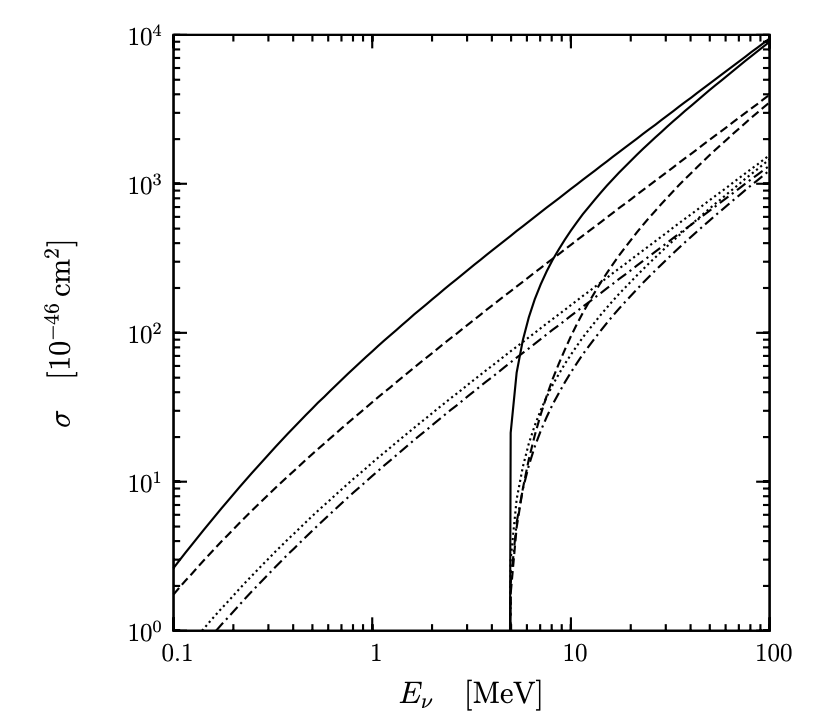
\includegraphics[width=0.6\linewidth]{nu_e_xsec}
  \caption{Electron neutrino cross-sections as a functions of the neutrino energy $E$. Solid line: $\nu_e+e^-\to\nu_e+e^-$. Dashed line: $\overline{\nu}_e+e^-\to\overline{\nu}_e+e^-$. Dotted line: $\nu_{\mu, \tau}+e^-\to\nu_{\mu, \tau}+e^-$. Dash-dotted line: $\overline{\nu}_{\mu. \tau}+e^-\to\overline{\nu}_{\mu. \tau}+e^-$. For each scattering process the upper curve is the cross-section without a threshold for the kinetic energy of the recoil electron, whereas the lower curve is obtained with $T_e^{th}=4.50 MeV$, which corresponds to $E_\nu^{th} = 4.74 MeV$. From~\cite{Auerbach2001}}
  \label{fig:intro:nue_xsec}
\end{figure}


\subsection{Interactions with nuclei}
\label{sec:intro:nuclei}
Neutrino interactions with a single fermion (e.g. quark) are very well known. But the atomic nuclei are complicated structures consisting of several particles that make the neutrino interaction description much more complicated. The reaction topology severely depends on the neutrino energy. The following energy scales can be set:
\begin{itemize}
  \item $E_\nu <$ 0.1 GeV: the neutrino interacts with the whole nucleus,
  \item $E_\nu\sim$ 0.1 -- 2 GeV: the neutrino interacts with one or few nucleons inside the nucleus,
  \item $E>$ few GeV: the neutrino interacts with the individual quarks
\end{itemize}

The energy scales above can be easily understood with De Broglie's wave approach. The incoming neutrino wavelength should be compared with the target's size.

From the experimental point of view, we can classify the neutrino interactions based on the outgoing particles. Thus we can divide all the reactions in the charged current and neutral current exchange. In the case of a charged current exchange, one will observe an outgoing charged lepton, while in case of neutral current exchange only hadrons and photons can be seen. Now we will define several topologies for the interactions via charged current. At the energies $\le1$ GeV neutrino mostly interacts in a quasi-elastic way (CCQE --- charge current quasi--elastic), transforming neutron into a proton. For the neutrinos with energies of 1 GeV the most probable reaction is a $\Delta^{++}$ production with its further decay into proton and pion. Also at this energy scale, we can see the coherent pion production, when a neutrino interacts with the whole nucleon or interactions with two nucleons simultaneously (2p2h interactions). With the energy growth, one will observe the dominance of the deep inelastic scattering with the various hadron production as a result of the broken nucleon. The Feynman diagrams for the processes mentioned above are shown in \autoref{fig:intro:f_nu_nucl}.

\begin{figure}[!ht]
  \centering
  \begin{minipage}{0.29\linewidth}
    \centering
    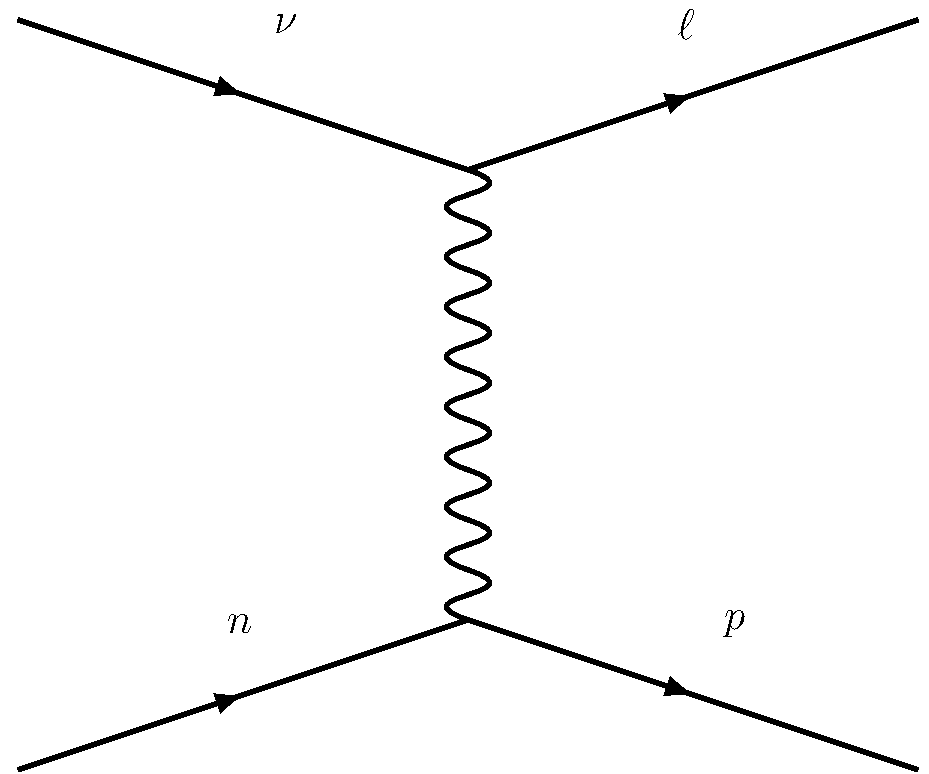
\includegraphics[width=0.8\linewidth]{f_nu_CCQE} \\ (a)
  \end{minipage}
  \begin{minipage}{0.29\linewidth}
    \centering
    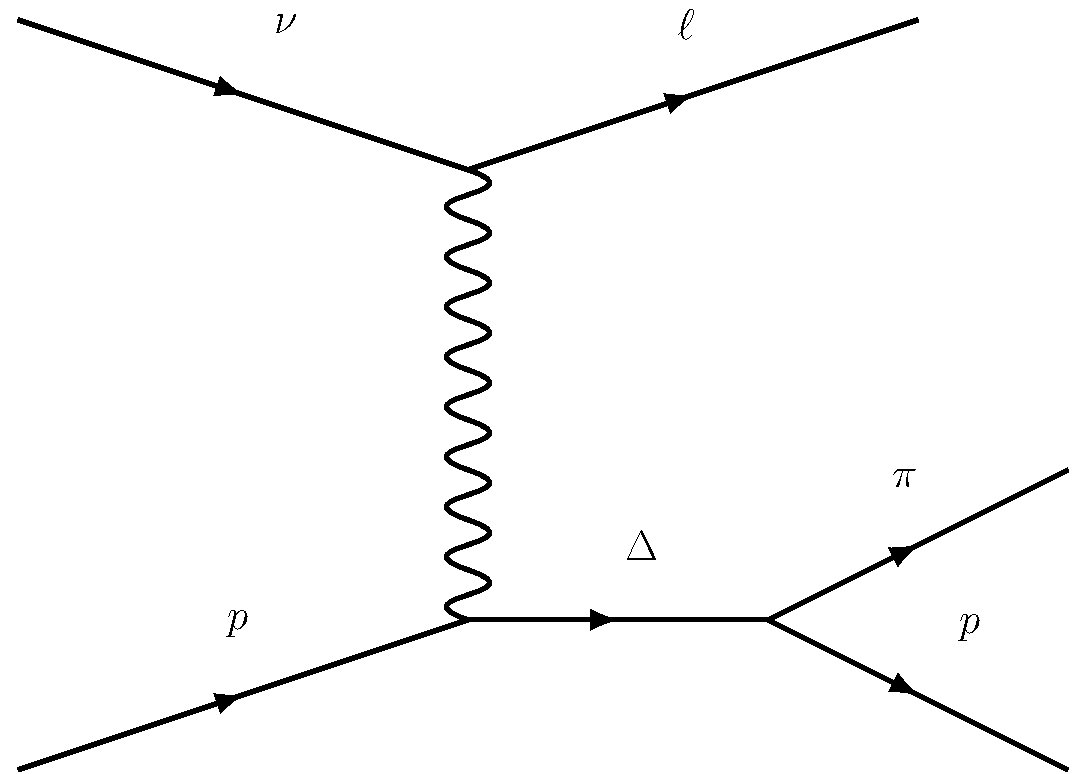
\includegraphics[width=0.8\linewidth]{f_nu_RES} \\ (b)
  \end{minipage}
  \begin{minipage}{0.29\linewidth}
    \centering
    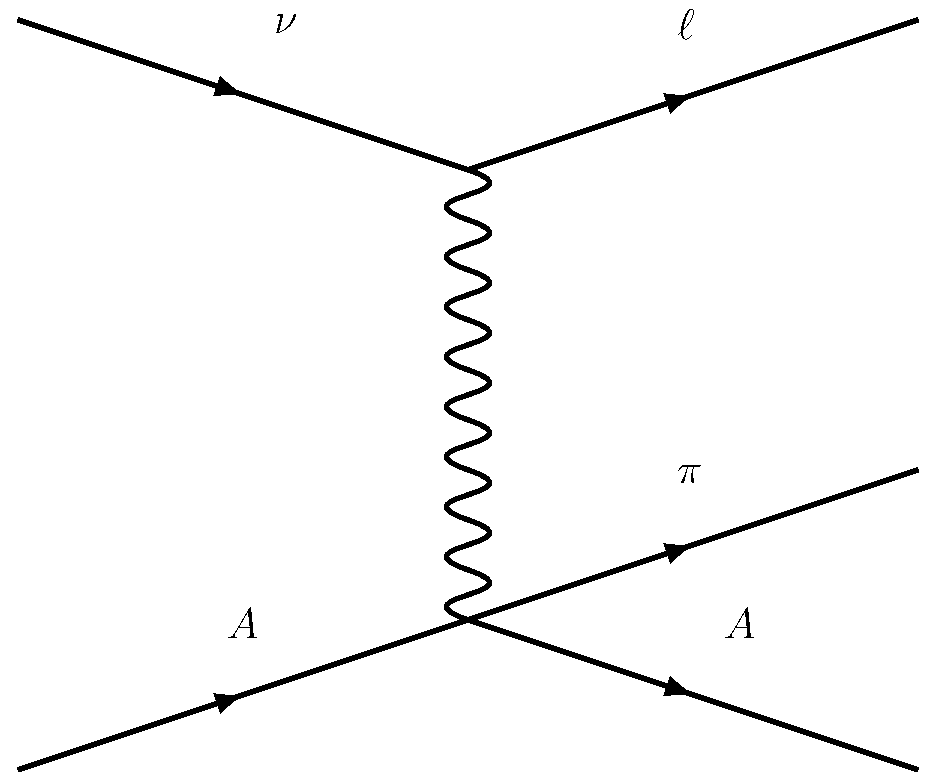
\includegraphics[width=0.8\linewidth]{f_nu_COH} \\ (c)
  \end{minipage}
  \vfill
  \begin{minipage}{0.29\linewidth}
    \centering
    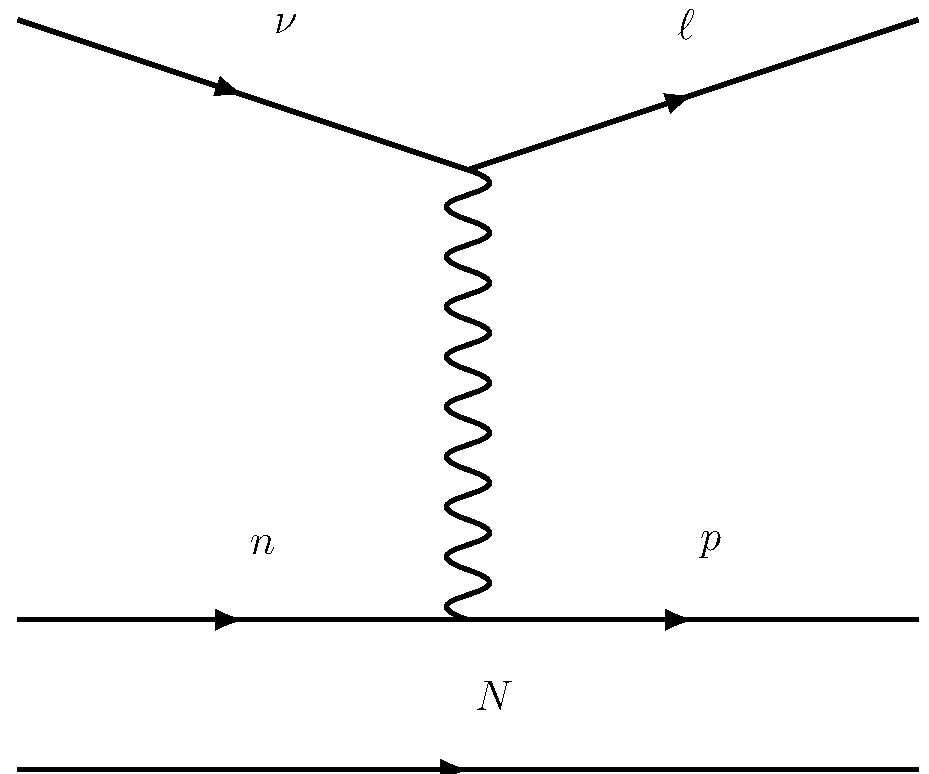
\includegraphics[width=0.8\linewidth]{f_nu_2p2h} \\ (d)
  \end{minipage}
  \begin{minipage}{0.29\linewidth}
    \centering
    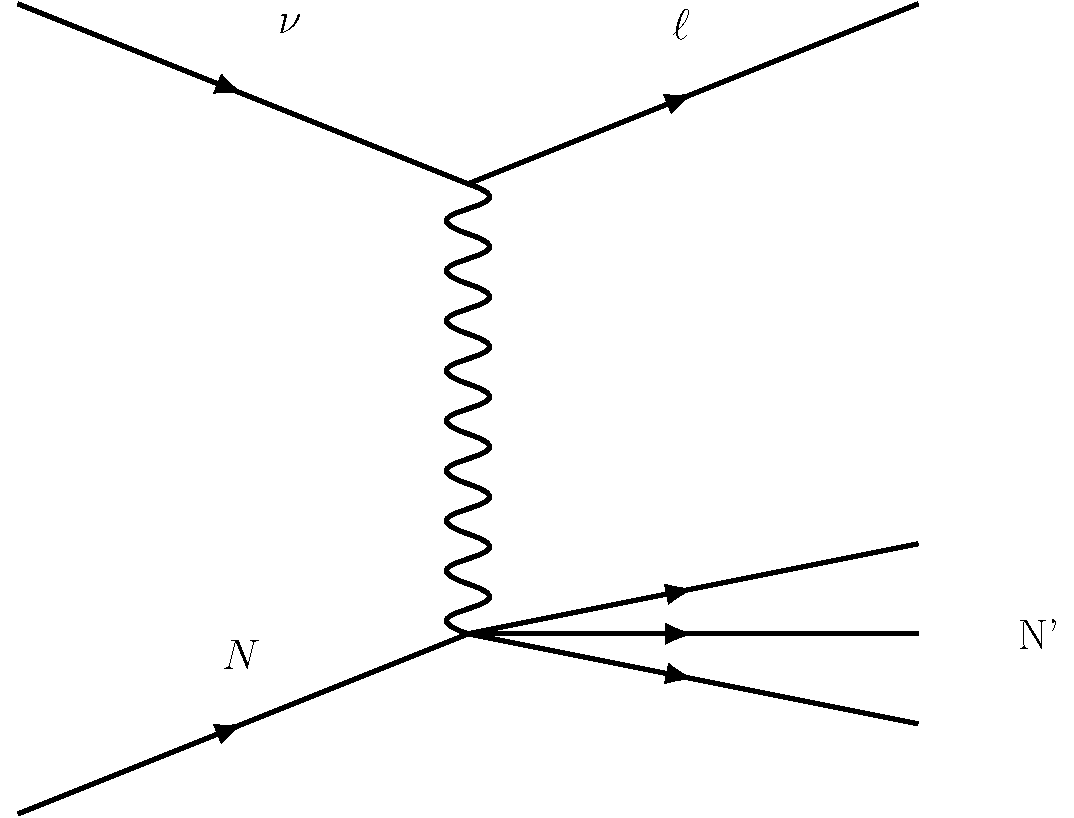
\includegraphics[width=0.8\linewidth]{f_nu_DIS} \\ (e)
  \end{minipage}
  \caption{Feynman diagrams for the neutrino interactions with nucleus. The following reactions are shown: (a) quasi elastic scattering, (b) resonance pion production, (c) coherent pion production, (d) 2p2h, (e) deep inelastic scattering.}
  \label{fig:intro:f_nu_nucl}
\end{figure}

The evaluation of the neutrino and anti-neutrino cross-sections with the energy is shown in \autoref{fig:intro:nu_xsec}.

\begin{figure}[!ht]
  \centering
  \begin{minipage}{0.49\linewidth}
    \centering
    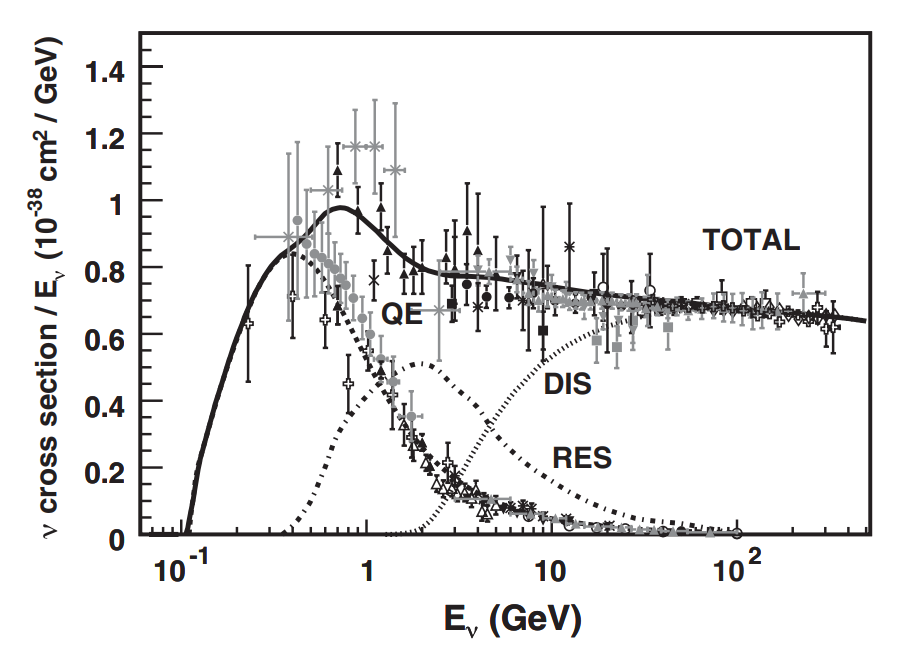
\includegraphics[width=\linewidth]{nu_xsec} \\ (a)
  \end{minipage}
  \begin{minipage}{0.49\linewidth}
    \centering
    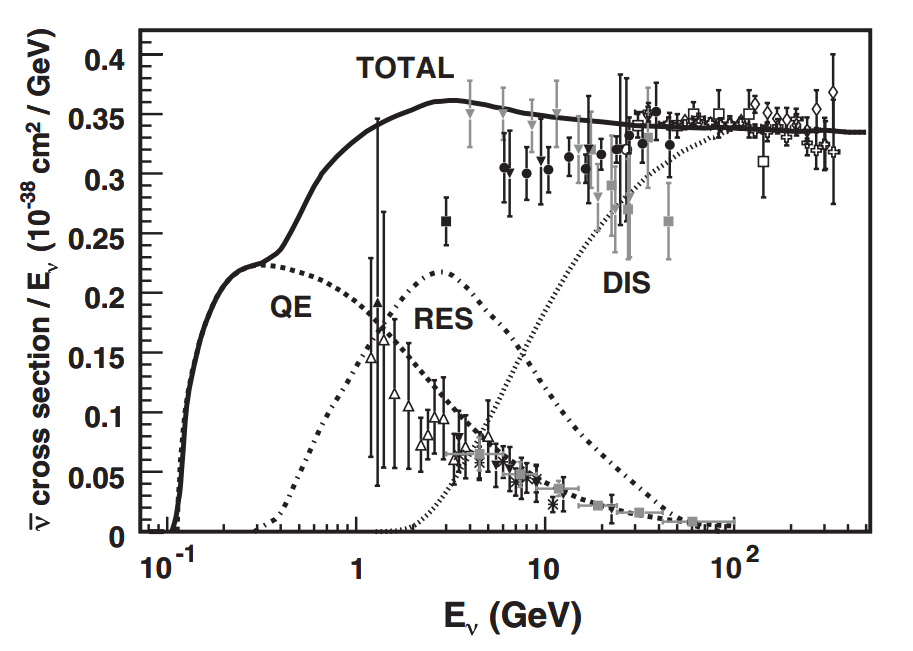
\includegraphics[width=\linewidth]{anu_xsec} \\ (b)
  \end{minipage}
  \caption{(a) neutrino and (b) anti-neutrino per nucleon CC cross sections from~\cite{Formaggio2012}.}

  \label{fig:intro:nu_xsec}
\end{figure}

Discussing the neutrino interaction with the nucleus it is worth mentioning the main experimental challenges. Above we discussed mostly the interactions on the single nucleon. While in fact, it happens only for targets made from Hydrogen. In most of the experiments, heavier targets are used. As a result, the neutrino interactions are affected by the following nuclear effects:
\begin{itemize}
  \item Fermi motion. The nucleons are not at rest inside the nucleus. This effect is called Fermi motion. Several models can be used to parametrize this phenomenon, e.g. Relativistic Fermi Gas (RFG) with the typical momentum depending on the nucleus. For example for Carbon $p_F\approx 220 MeV/c^2$,
  \item Final State Interactions (FSI). After the initial neutrino reaction, final state particles such as pions or nucleon can interact while propagating inside the nucleus. For example, the pion can be absorbed, or additional hadrons can be produced.
  \item collective effects. The neutrino can interact with several nucleons at the same time. The most common case is the interaction with 2 particles -- 2p2h (2 particles, 2 holes). As the models of nucleons interactions are not precise enough this effect introduces relatively large uncertainty in the analysis.
\end{itemize}

The detailed description of the neutrino-nucleus interactions can be found in~\cite{Formaggio2012}.

% \subsection{Transverse kinematic variable}
% \label{sec:intro:pt}
% The nuclear effects implement large uncertainties in the measurements of neutrino energy. To avoid the uncertainties one can try to select a particular kinematic sample that is free or at least depends poorly on the nuclear effects. Such a sample can be selected with so--called transverse kinematic variables. For CC0$\pi$ interactions

% \cite{Lu2016}

% \begin{figure}[!ht]
% 	\centering
%     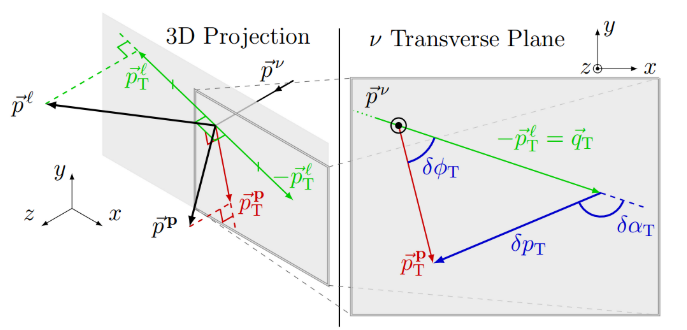
\includegraphics[width=0.6\linewidth]{pt_schema}
%     \caption{Schematic view of the definition of the observables: $\delta p_T$, $\delta \alpha_T$, and $\delta\phi_T$.}
%     \label{fig:intro:pt_schema}
% \end{figure}

% \begin{figure}[!ht]
%   \centering
%   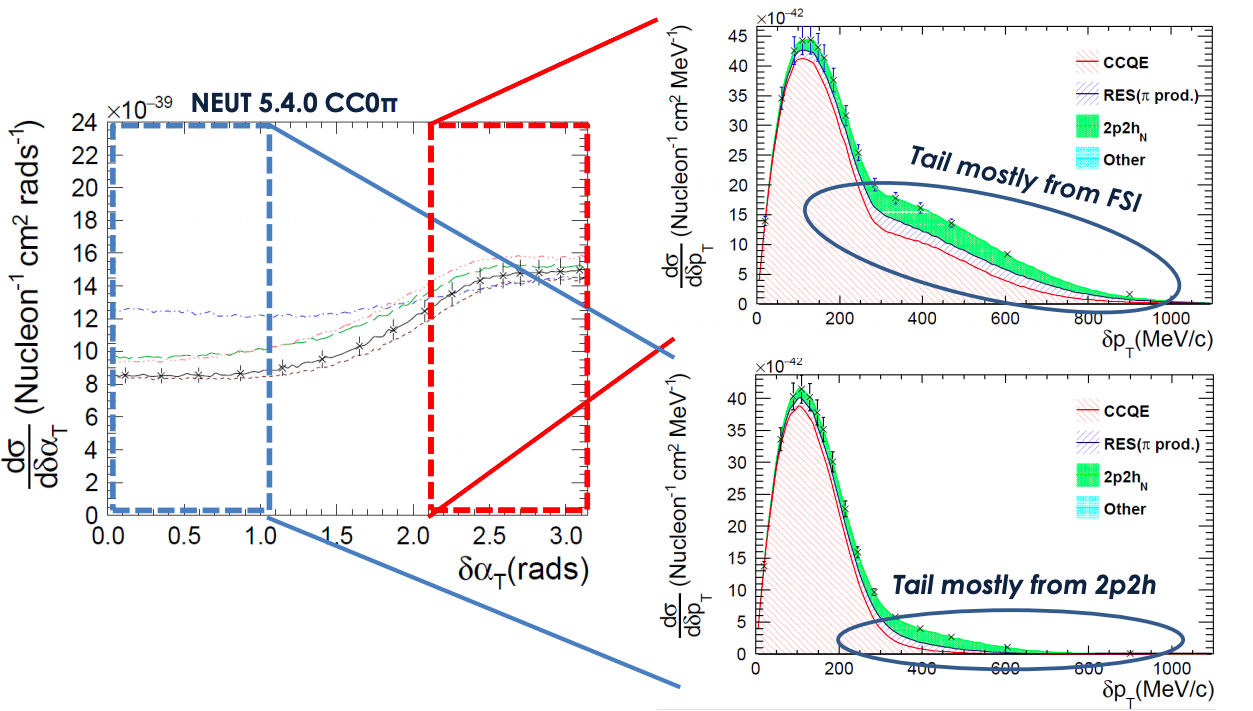
\includegraphics[width=0.8\linewidth]{dpt_spectra}
%   \caption{The illustration of probing nuclear effects in the different bins of tracsverse variables.}
%   \label{fig:intro:pt_spectra}
% \end{figure}

\section{Neutrino oscillations}
\label{sec:intro:osc}
The neutrino oscillation phenomenon research started with the phenomenological prediction, followed by the puzzle of the small neutrino flux from the Sun. A milestone was reached recently with the robust confirmation of the effect. Many interesting discoveries were made during the oscillation analysis, e.g. non-zero neutrino mass, large mixing angles, hints for the CP--violation; many different ways to produced and study neutrinos were found. But many results are still awaiting. In this section, the modern understanding of the phenomenon will be presented as well as the latest experimental results.

\subsection{Theory}
The experimental confirmation that neutrino and anti-neutrino interact differently came soon after neutrino discovery. Inspired by the observed oscillations of neutral kaons $K^0\to\overline{K^0}$ Bruno Pontecorvo proposed the oscillations $\nu\to\bar\nu$~\cite{Pontecorvo1957}. For such process neutrino should have small but non-zero mass. At that time the experimental confirmation of such a hypothesis was very challenging as the effect can not be measured in the laboratory but with cosmological observations only.

After the discovery of the muon neutrino, a different hypothesis of the neutrino flavor oscillations $\nu_e\to\nu_\mu$ was proposed. Maki, Nagava and Sakata developed a theory of the 2-flavor neutrino oscillations~\cite{Maki1962}.

\subsubsection{Phenomenology}
The phenomenology of the neutrino oscillation will be described below with the quantum mechanics approach for 3 neutrino flavors. The state of the neutrino can be described either with a flavor basis $\lvert\nu_\alpha\rangle$ or with a mass basis $\lvert\nu_k\rangle$. The relation between them is defined by the mixing matrix $U_{\alpha k}$.

\begin{equation}
\label{eq:intro:mixing}
\lvert\nu_\alpha\rangle = \sum_kU^*_{\alpha k}\lvert\nu_k\rangle
\end{equation}
where $\alpha = e, \mu, \tau$ and $k=1, 2, 3$. Thus the mixing between the flavor and mass states of the leptons are allowed. We measure the flavor of both produced and interacted neutrino with the flavor of the accompanying charged lepton. But the propagation of the particle is defined by its mass. Within the quantum mechanics approach the Schroedinger equation will describe the changes of the system with time.

\begin{equation}
i\frac{d}{dt}\lvert\nu_k(t)\rangle=\mathcal{H}\lvert\nu_k\rangle
\end{equation}
where the Hamiltonian of the system is such that
\begin{equation}
\label{eq:intro:ham}
\mathcal{H}\lvert\nu_k\rangle=E_k\lvert\nu_k\rangle
\end{equation}

The changes with time will be described by the evolution of the operator
\begin{equation}
\label{eq:intro:evol}
\lvert\nu_k(t)\rangle=e^{-iE_kt}\lvert\nu_k\rangle
\end{equation}

As was mentioned above the production and detection of the neutrino should be described by the flavor states. Modifying \autoref{eq:intro:evol} with \autoref{eq:intro:mixing} we will get
\begin{equation}
\lvert\nu_\alpha(t)\rangle=\sum_{\beta=e, \mu, \tau}\left(\sum_k U^*_{\alpha k}e^{-iE_kt}U_{\beta k} \right)\lvert\nu_\beta\rangle
\end{equation}

The oscillation probability is the square of the matrix element

\begin{align}
P_{\nu_\alpha\to\nu_\beta}&=\left|A_{\nu_\alpha\to\nu_\beta}(t)\right|^2=\left|\langle\nu_\beta\vert\nu_\alpha(t)\rangle\right|^2 \\ \nonumber
{}&=\sum_{k, j}U^*_{\alpha k}U_{\beta k}U_{\alpha j}U^*_{\beta j}e^{-i\left(E_k-E_j\right)t}
\end{align}

Neutrino masses are expected to be extremely small $\leqslant 1eV$ while we want to describe the energy scale above a few keV. In this case, an ultra-relativistic approximation is applicable.
\begin{align}
E_k-E_j \simeq&\frac{\Delta m_{kj}^2}{2E} \\
&\Delta m_{kj}^2 \equiv m^2_k-m^2_j \nonumber
\end{align}
Thus the oscillation probability versus the travel distance and neutrino energy will be defined as

\begin{equation}
P_{\nu_\alpha\to\nu_\beta}(L, E)=\sum_{k, j}U^*_{\alpha k}U_{\beta k}U_{\alpha j}U^*_{\beta j}\exp\left(-i\frac{\Delta m^2_{kj}L}{2E}\right)
\end{equation}

The neutrino oscillations can be classified into two major types:
\begin{itemize}
  \item ``disappearance'' --- the phenomenon of observation of less neutrino with a given flavor comparing to the produced amount
  \item ``appearance'' --- the phenomenon of the observation of neutrino flavor which was not initially produced, e.g. $\nu_e$, while  only $\nu_\mu$ was produced
\end{itemize}
There is a common practice to split the real and imaginary part of the oscillation probability as they will demonstrate different behavior. For example, the real part is CP conservative, while the imaginary part violates CP symmetry. The ``appearance'' probability will be calculated with
\begin{align}
\nonumber
P_{\nu_\alpha\to\nu_\beta}(L, E)=\delta_{\alpha\beta}&-4\sum_{k>j}\mathfrak{Re}\left[U^*_{\alpha k}U_{\beta k}U_{\alpha j}U^*_{\beta j}\right]\sin^2\left(\frac{\Delta m^2_{kj}L}{4E}\right) \\
&+2\sum_{k>j}\mathfrak{Im}\left[U^*_{\alpha k}U_{\beta k}U_{\alpha j}U^*_{\beta j}\right]\sin\left(\frac{\Delta m^2_{kj}L}{2E}\right)
\label{eq:intro:app}
\end{align}

In its turn, the ``disappearance'' phenomenon will be described by
\begin{equation}
\label{eq:intro:dis}
P_{\nu_\alpha\to\nu_\alpha}(L, E)=1-4\sum_{k>j}\left|U_{\alpha k}\right|^2\left|U_{\alpha j}\right|^2\sin^2\left(\frac{\Delta m^2_{kj}L}{4E}\right)
\end{equation}

\begin{bclogo}[couleur=blue!2, arrondi=0.1, logo=\bcinfo, nobreak=true]{Mixing matrix unitarity}
In this section we assumed the unitarity of the mixing matrix
\begin{equation}
U^\dag U=1 \Longleftrightarrow\sum_\alpha U^*_{\alpha k}U_{\alpha j}=\delta_{jk}
\end{equation}

This assumption came from the fundamental laws of QFT. And it indeed should be true for mixing matrix of any dimension. As will be described in \autoref{ch:intro:HNL} the model with 3x3 mixing matrix is not essential for the explanation of the neutrino mass. In this case, due to the existence of other neutrino states the mixing matrix of 3 left-handed neutrino is not unitary.

\begin{equation}
\sum_{\alpha=e, \mu, \tau} U^*_{\alpha k}U_{\alpha j}\neq\delta_{jk}
\end{equation}
At the moment there is no experimental confirmation of this effect.
\end{bclogo}

\subsubsection{Mixing matrix parametrization}
In this subsection, we will describe the most common parametrization of the 3-flavor neutrino mixing matrix. This matrix was named Pontecorvo-Maki-Nagava-Sakata in memory of the pioneers of the oscillation theory. In the common representation, the matrix consists of 9 elements

\begin{equation}
\begin{pmatrix}
\nu_e \\ \nu_\mu \\ \nu_\tau
\end{pmatrix}
=
\begin{pmatrix}
U_{e1} & U_{e2} & U_{e3} \\
U_{\mu 1} & U_{\mu 2} & U_{\mu 3} \\
U_{\tau 1} & U_{\tau 2} & U_{\tau 3} \\
\end{pmatrix}
\begin{pmatrix}
\nu_1 \\ \nu_2 \\ \nu_3
\end{pmatrix}
\end{equation}
for easier parametrization, it is usually written as a multiplication of four matrices

\begin{align}
\nonumber
U=&
\begin{pmatrix}
1   & 0                 & 0 \\
0   & \cos\theta_{23}   & \sin\theta_{23} \\
0   & -\sin\theta_{23}  & \cos\theta_{23}
\end{pmatrix}
\times
\begin{pmatrix}
\cos\theta_{13}                           & 0     & \sin\theta_{13}e^{-i\delta} \\
0                                         & 1     & 0 \\
-\sin\theta_{13}e^{+i\delta}              & 0     & \cos\theta_{13}
\end{pmatrix} \times \\
\times &
\begin{pmatrix}
\cos\theta_{12}   & \sin\theta_{12} & 0 \\
-\sin\theta_{12}  & \cos\theta_{12} & 0 \\
0                 & 0               & 1
\end{pmatrix}
\times
\begin{pmatrix}
\exp\frac{i\alpha_1}{2}   & 0                         & 0 \\
0                         & \exp\frac{i\alpha_2}{2}   & 0 \\
0                         &                           & 1
\end{pmatrix}
\label{eq:intro:osc_param}
\end{align}

Such parametrization is done with three mixing angles: $\theta_{12}, \theta_{13}, \theta_{12}$ and three CP-violating phases: $\delta$ and $\alpha_1$, $\alpha_2$. The mixing angles define the transition from the mass state basis to the flavor state basis. The schema of these rotations is shown in \autoref{fig:intro:basis}.

\begin{figure}[!ht]
  \centering
  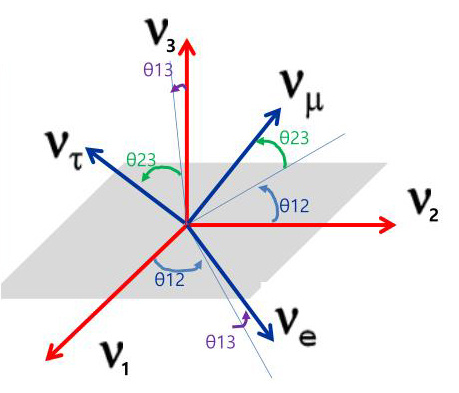
\includegraphics[width=0.4\linewidth]{basis.jpg}
  \caption{Reference rotation of the flavor basis versus the mass basis. The corresponding mixing angles are shown.}
  \label{fig:intro:basis}
\end{figure}


Before rewriting the equations \ref{eq:intro:app} and \ref{eq:intro:dis} with the new parametrization, let me specify the following notations

\begin{equation}
c_{ij}=\cos\theta_{ij} \hspace{3cm} s_{ij}=\sin\theta_{ij}
\end{equation}
\begin{align}
\nonumber
\Delta_{reactor} \equiv \Delta_{13} = \frac{\Delta m^2_{13}L}{4E_\nu} \\
\Delta_{solar} \equiv \Delta_{21} = \frac{\Delta m^2_{21}L}{4E_\nu} \\
\Delta_{atm} \equiv\Delta_{32} = \frac{\Delta m^2_{32}L}{4E_\nu} \nonumber
\end{align}

The $\Delta_{13}$, $\Delta_{21}$ and $\Delta_{32}$ terms are referred as reactor, solar and atmospheric oscillation phases. The impact of these phases is dominating at the neutrino energies and ranges typical for the mentioned sources. The mixing angles and mass differences can be also referred based on the experiments where they are dominating. For example, $\theta_{13}$ and $\Delta m^2_{13}$ are called reactor oscillation parameters. The accelerator neutrino experiments are sensitive to both reactor and atmospheric parameters.

With the defined notation the $\nu_\mu$ disappearance probability can be written:

\begin{equation}
\begin{split}
P_{\nu_\mu\to\nu_\mu}=&1-\left(c^4_{13}\sin^22\theta_{23} + s^2_{23}\sin^22\theta_{13}\right)\sin^2\Delta_{13} \\
+&\left\{c_{13}^2\left(c^2_{12}-s^2_{13}s^2_{23}\right)\sin^22\theta_{23}+s^2_{12}s^2_{23}\sin^22\theta_{13}-c_{13}\sin2\theta_{13}\sin2\theta_{23}\sin2\theta_{12}\cos\delta\right\} \\
\times&\left\{\frac{1}{2}\sin2\Delta_{21}\sin2\Delta_{13}+2\sin^2\frac{\Delta m_{21}^2L}{4E_\nu} + 2\sin\Delta_{21}\sin^2\Delta_{13}\right\} \\
-&\left\{\sin^22\theta_{12}\left(c^2_{23}-s^2_{13}s^2_{23}\right)^2+s_{13}^2\sin^22\theta_{23}\left(1-\cos\delta^2\sin^22\theta_{12}\right) \right.\\
+&2s_{13}\sin2\theta_{12}\cos2\theta_{12}s_{23}\cos2\theta_{23}\cos\delta \\
-&\frac{1}{2}c_{13}\sin2\theta_{13}\sin2\theta_{23}\sin2\theta_{12}\cos\delta s^2_{23}s^2_{12} \\
 +&\sin^22\theta_{23}c^2_{13}\left(c^2_{12}-\left. {}s^2_{13}s^2_{12}\right)+s^2_{13}s^2_{23}\sin^22\theta_{13} \vphantom{\left(\sin^22\theta_{12}\right)^2} \right\}\times\sin^2\Delta_{21}
\end{split}
\label{eq:intro:disapp_p}
\end{equation}

The formula above is quite complicated but it can be simplified for each particular experiment. For example, for an accelerator experiment with a neutrino beam with energies around 1 GeV (e.g. T2K experiment) and with latest results of the parameters measurements (\autoref{tbl:intro:osc}) the phases $\sin^2\Delta_{21}\approx0$ and $\sin2\Delta_{32}\approx0$. As a result the probability can be rewritten as:

\begin{equation}
\label{eq:intro:numu_simple}
P\left(\nu_\mu\to\nu_\mu\right)\approx1-\left(cos^4\theta_{13}\sin^22\theta_{23}+\sin^22\theta_{13}\sin^2\theta_{23}\right)\sin^2\frac{\Delta m^2_{31}L}{4E_\nu}
\end{equation}

The first term in the brackets is the leading one and the following is next-to-leading. It is important to highlight that the probability will not change for the anti-neutrino disappearance ($\overline{\nu}_\mu\to\overline{\nu}_\mu$). Also, the phase $\delta_{CP}$ is severely suppressed in \autoref{eq:intro:disapp_p}.

The full probability for the $\nu_e$ appearance will be given by

\begin{equation}
\begin{split}
P_{\nu_\mu\to\nu_e}= &4c_{13}^2s_{13}^2s_{23}^2\sin\Delta_{13} \\
+&8c_{13}^2s_{12}s_{13}2_{23}\left(c_{12}c_{23}\cos\delta-s_{12}s_{13}s_{23}\right)\cos\Delta_{32}\sin\Delta_{13}\sin\Delta_{21} \\
-&8c_{13}^2c_{12}c_{23}s_{12}S_{13}S_{23}\sin\delta\sin\Delta_{32}\sin\Delta_{31}\sin\Delta_{21} \\
+&4s_{12}^2c_{13}^2\left(c_{12}^2c^2_{23}+s^2_{122}s^2_{23}s^2_{13}-2c_{12}c_{23}s_{12}s_{23}s_{13}\cos\delta\right)\sin^2\Delta_{21}
\end{split}
\label{eq:intro:app_p}
\end{equation}

The probability for the anti-neutrino oscillation will be obtained with the change $\delta\to-\delta$. The second line is invariant under this transformation while the third one will be the opposite. It means that neutrino and anti--neutrino oscillate differently. This effect can be observed only in the appearance channel. The importance of such a phenomenon is described in the next subsection.

As for the muon disappearance, the appearance formula can be quite simplified. The first term is the leading one. For the accelerator experiment with 1 GeV neutrino beam the probability around the 1st oscillation maximum can be estimated with the leading and CP--odd term.

\begin{align}
\label{eq:intro:nue_simple}
P\left(\nu_\mu\to\nu_e\right)\approx&\sin^2\theta_{23}\sin^2\theta_{13}\sin^2\frac{\Delta m_{32}^2L}{4E_\nu} \\
-&\sin2\theta_{12}\sin2\theta_{13}\cos\theta_{13}\sin\delta\sin^2\frac{\Delta m_{32}^2L}{4E_\nu}\sin\frac{\Delta m_{21}^2L}{4E_\nu}
\end{align}

The visualization of the formulas above is provided in \autoref{fig:intro:osc2} (\autoref{fig:intro:osc1} and \autoref{fig:intro:osc3} for initial electron and tau neutrino beam respectively). The oscillation curves for each initial state ($e, \mu, \tau$) and two $E/L$ are shown. From such a plot, it is much easier to understand the meaning of the oscillation parameters. The mixing angles define oscillation amplitude and the mass difference defines frequency.

\begin{figure}[!ht]
\centering
\begin{minipage}{0.4\linewidth}
  \centering
  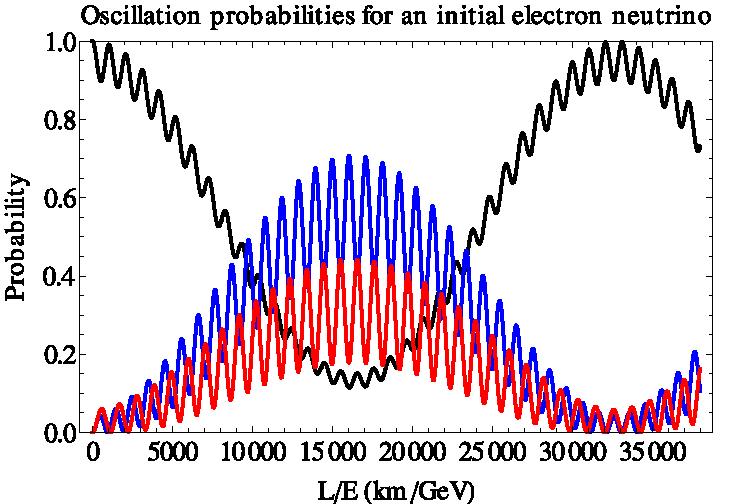
\includegraphics[width=\linewidth]{osc_ele_large}
\end{minipage}
\hfill
\begin{minipage}{0.4\linewidth}
  \centering
  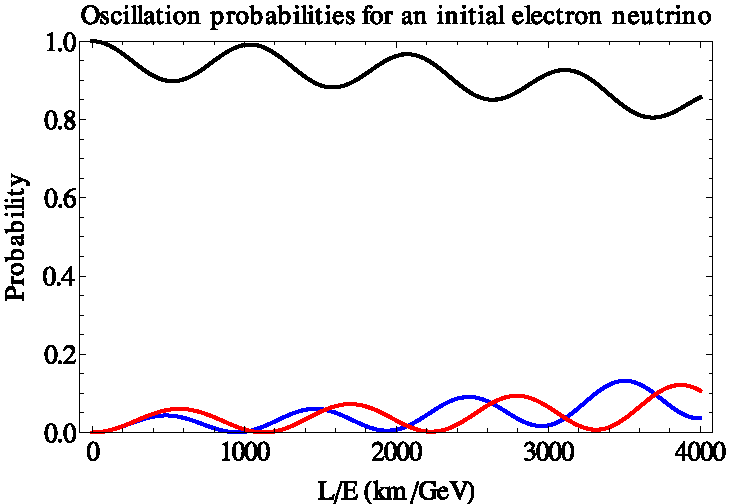
\includegraphics[width=\linewidth]{osc_ele_short}
\end{minipage}
\caption{Oscillation probabilities for the initial electron neutrino state for two different L/E scales. The black line corresponds to the electron neutrino component, blue line for muon neutrino and red line for tau neutrino.}
\label{fig:intro:osc1}
\end{figure}

\begin{figure}
\centering
\begin{minipage}{0.4\linewidth}
  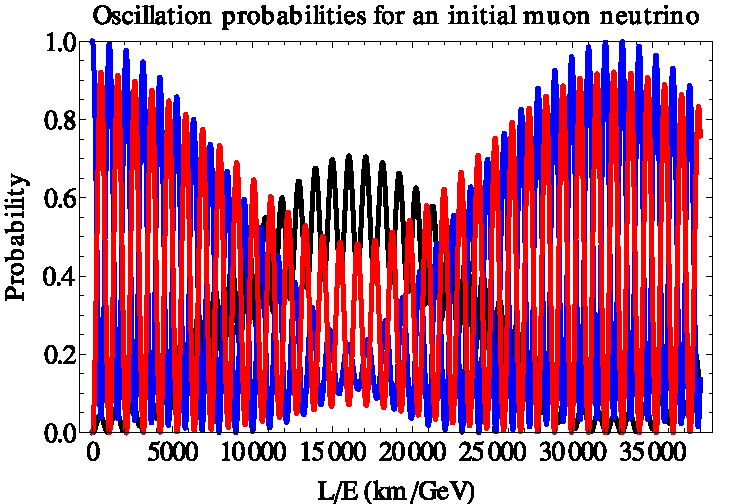
\includegraphics[width=\linewidth]{osc_muon_large}
\end{minipage}
\hfill
\begin{minipage}{0.4\linewidth}
  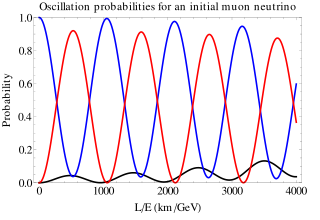
\includegraphics[width=\linewidth]{osc_muon_short}
\end{minipage}
\caption{Oscillation probabilities for the initial muon neutrino state for two different L/E scales. The black line corresponds to the electron neutrino component, blue line for muon neutrino and red line for tau neutrino.}
\label{fig:intro:osc2}
\end{figure}

\begin{figure}
\centering
\begin{minipage}{0.4\linewidth}
  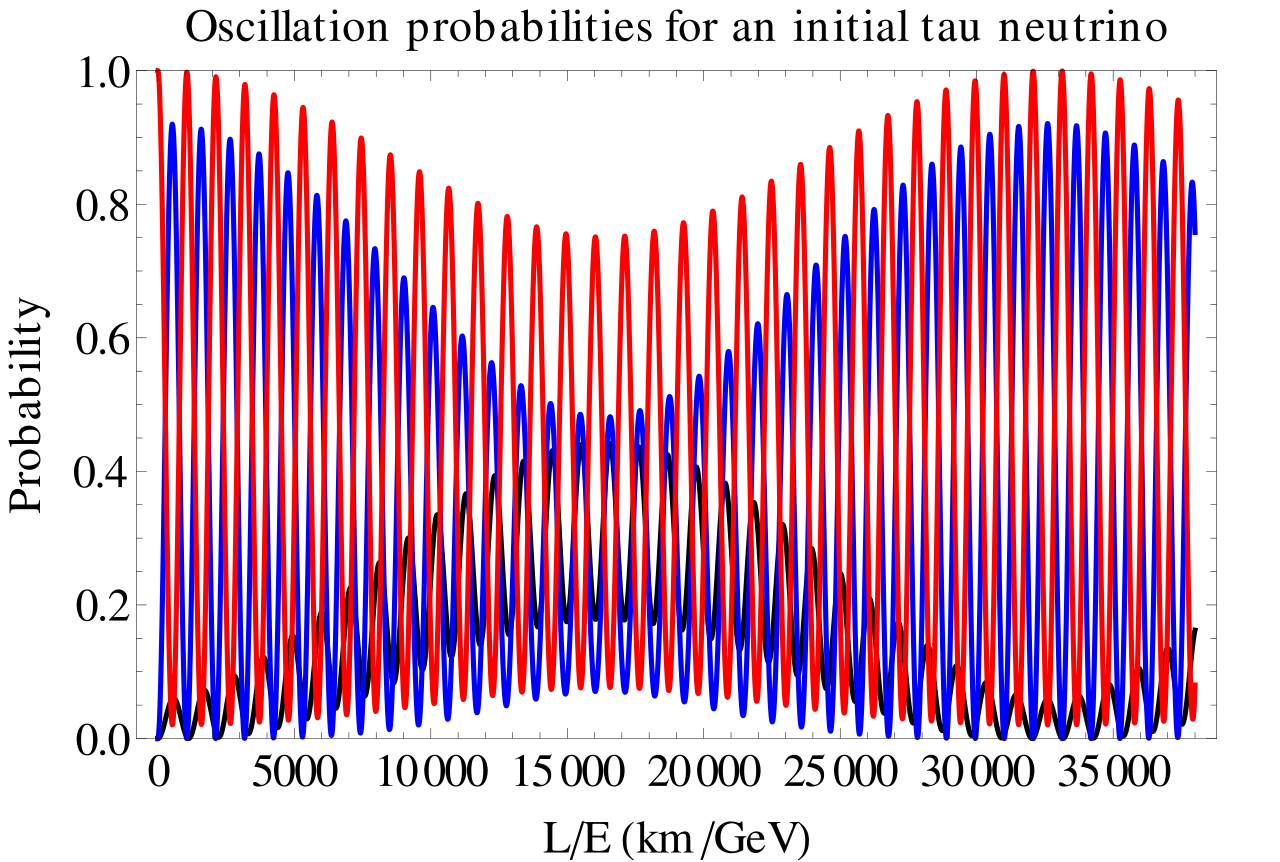
\includegraphics[width=\linewidth]{osc_tau_large}
\end{minipage}
\hfill
\begin{minipage}{0.4\linewidth}
  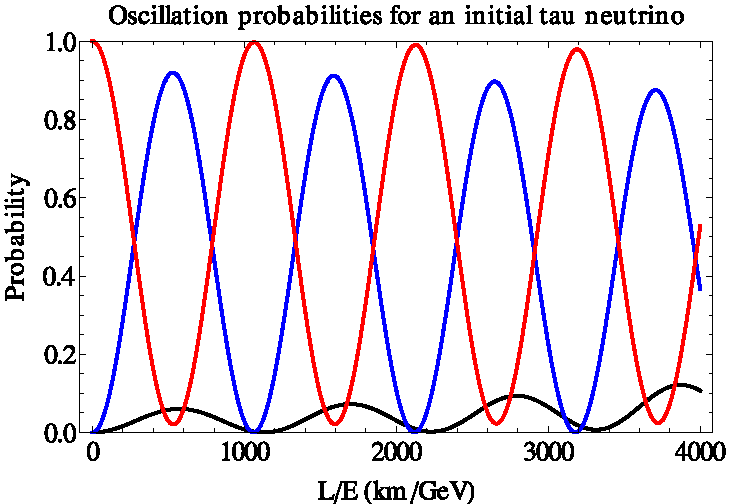
\includegraphics[width=\linewidth]{osc_tau_short}
\end{minipage}
\caption{Oscillation probabilities for the initial tau neutrino state for two different L/E scales. The black line corresponds to the electron neutrino component, blue line for muon neutrino and red line for tau neutrino.}
\label{fig:intro:osc3}
\end{figure}

\subsubsection{CP violation in the neutrino oscillations}
\label{sec:intro:cp}
The phenomenon of the CP--violation in the neutrino oscillation is worth emphasizing. The dominance of matter over the anti-matter was observed in the Universe. Modern cosmology faces the problem of explaining such a phenomenon. The fundamental conditions for the matter-dominance generation were developed by Sakharov~\cite{Sakharov1967}. One of the key conditions is CP--violation. This phenomenon was observed in the quark sector~\cite{Tanabashi2018}. But the precise measurements show that the amplitude of the CP--violation is not sufficient to generate the observed asymmetry in the Universe.

Several models propose the generation of the matter dominance through the lepton sector~\cite{Davidson2008}. The non-zero CP-violation phase (\autoref{eq:intro:osc_param}) is required for such an effect. From the \autoref{eq:intro:disapp_p} and \autoref{eq:intro:app_p} we can clearly see that the CP-violating phase can be measured only in the appearance channel and the total effect is scaled by the value of the mixing angle $\theta_{13}$. According to the latest measurements, the value of the $\theta_{13}$ mixing angle is not zero that allows the direct search for the leptonic CP-violation in the experiment.

The latest results of the CP--violation measurements in the neutrino oscillations will be presented in \autoref{sec:intro:osc_exp}. It is important to note that the CP--violation in the mixing of three known neutrino generations is not the only essential condition to generate the matter-dominance in the early Universe. The existence of heavy neutrinos (\autoref{sec:intro:HNL}) is also necessary.

\begin{bclogo}[couleur=blue!2, arrondi=0.1, logo=\bcinfo, nobreak=true]{Transformations: C, P, T}
In particle physics there are three important transformations: charge (C), parity (P) and time (T).

Parity inversion (P) flips the sign of the spatial coordinate $\mathcal{P}\overrightarrow{r}=-\overrightarrow{r}$ . In the QFT it is described as $\mathcal{P}\lvert\psi\rangle=c\lvert\psi\rangle$ where $c$ is the eigenvalue of $\mathcal{P}$. The parity violation means a process that changes the eigenvalue of the parity transformation for some system. The theoretical possibility of such a process was found by Lee and Yang~\cite{Lee1956} and proved in the Wu's experiment~\cite{Wu1957}. The asymmetry of the outgoing electrons from the Cobalt with respect to the nucleus polarization was the nice and clear proof for the effect.

Charge transformation (C) changes a particle to its anti-particle. $\mathcal{C}\lvert\psi\rangle=\eta_{C}\lvert\bar{\psi}\rangle$, where $\eta_{C}$ is the eigenvalue of the transformation. The example of the eigenvalue non-conservation experimental observation can be found in~\cite{Gormley1968}.

Time transformation (T) inverses the time direction. After the discovery of the separate P and C violations, the combined symmetry breaking was looked for. As it will be a hint towards T-symmetry breaking. CP--violation was observed in the neutral kaons oscillations process~\cite{Christenson1964}. Later such a process was confirmed with the direct measurements of kaon decays~\cite{Alavi-Harati1999}~and~\cite{Fanti1999}, B-meson decays~\cite{Aubert2001}~and~\cite{Abe2001}, D-mesons~\cite{Aaij2019}.

It has been demonstrated that any Lorentz invariant local quantum field theory with a hermitian Hamiltonian must be invariant under CPT.
\end{bclogo}

\subsubsection{2--flavor oscillations}
In the previous section, the modern framework of the neutrino oscillations was described. Historically the neutrino mixing theory was developed for 2 flavors. While 3-flavor oscillation probability equations are quite complicated, a 2--flavor approximation often provides sufficient accuracy and suitable for the many experiments. In this approach, the mixing matrix becomes a usual $2\times2$ rotation matrix
\begin{equation}
U=
\begin{pmatrix}
\cos\theta    & \sin\theta     \\
-\sin\theta   & \cos\theta
\end{pmatrix}
\end{equation}
and the oscillation probabilities will be written as

\begin{align}
P_{\nu_\alpha\to\nu_\alpha}=1-&\sin^22\theta\sin^2\frac{1.27\Delta m^2L}{E_\nu} \\
P_{\nu_\alpha\to\nu_\beta}=&\sin^22\theta\sin^2\frac{1.27\Delta m^2L}{E_\nu}
\end{align}
In this notation the neutrino energy unit is supposed to be GeV, the distance unit is km and the mass difference unit is $\text{eV}^2/\text{c}^4$.

\subsubsection{Oscillation in matter}
\label{sc:intro:mat}
The framework presented above, describes the oscillations in vacuum. In the case of neutrino propagation in matter, the effect will be different. Going through a medium neutrino suffers from the forward elastic scattering with electrons and nucleons. This effect is similar to the phenomenon of light propagation in the matter. A new potential which is equivalent to the refraction index needs to be taken into account. But the interaction types are slightly different for different neutrinos. All neutrino types may scatter on electrons, protons and neutrons through the neutral current exchange. Also, electron neutrino scatters on the electrons with the charge current. The framework of the neutrino oscillations in matter was developed by Wolfenstein~\cite{Wolfenstein1978}. The mixing angle and the mass difference should be replaced by the effective ones, depending on the matter density.


Describing the neutrino propagation in matter one needs to modify the Hamiltonian function from \autoref{eq:intro:ham}. In addition to the neutrino energy, the potential of the neutrino interactions with electron should be added.
\begin{equation}
H_{i,j}=\left(E_\nu+\frac{m_i^2}{2E_\nu}\right)\delta_{i,j}+U_{ei}^*U_{ej}\sqrt2G_Fn_e
\end{equation}
where $U$ is the neutrino mixing matrix, $G_F$ is the Fermi constant and $n_e$ is the electron density in matter. For the simplification, I will estimate the changing of the oscillation parameters in the 2--flavor framework in matter with a constant density. In vacuum, the mixing angle and the mass difference are defined with $\theta$ and $\Delta m^2$ parameters. The new effective values in matter can be written  as:
\begin{align}
\sin^22\theta_M&=\frac{\sin^22\theta}{\cos^22\theta(1-\lambda)^2+\sin^22\theta} \\
\Delta m^2_M&=\Delta m^2\frac{\sin2\theta}{\sin2\theta_M} \\
\lambda&=\frac{2\sqrt2G_FE_\nu n_e}{\Delta m^2\cos2\theta}
\end{align}

In the case of a slightly changing density of matter, there is a region where the mixing angle reaches its maximum possible value $\pi/4$~\cite{Mikheyev1985}. This phenomenon is called Mikheyev–-Smirnov–-Wolfenstein (MSW) effect.

The effect of the oscillations in matter is quite small in the reactor experiments but not negligible in accelerator experiments. The beam is traveling hundreds of kilometers through the matter. The effect is more dramatic with the longer baseline. The disappearance channel ($\nu_\mu\to\nu_\mu$) is nearly unaffected by the presence of matter, but the appearance probability  ($\nu_\mu\to\nu_e$) will change. For the accelerator experiment with 1 GeV neutrino beam, the \autoref{eq:intro:nue_simple} will be updated with

\begin{align}
P\left(\nu_\mu\to\nu_e\right)\approx&\sin^2\theta_{23}\sin^2\theta_{13}\sin^2\frac{\Delta m_{32}^2L}{4E_\nu}\left(1+\frac{2a}{\Delta_{31}^2}\left(1-2\sin^2\theta_{13}\right)\right) \\
-&\sin2\theta_{12}\sin2\theta_{13}\cos\theta_{13}\sin\delta\sin^2\frac{\Delta m_{32}^2L}{4E_\nu}\sin\frac{\Delta_{21}^2L}{4E_\nu}
\end{align}

where $a\equiv2\sqrt(2)G_Fn_eE=7.56\times10^{-5}eV^2\frac{\rho}{gcm^2}\frac{E}{GeV}$. The effect for the anti--neutrino is opposite, so $a$ will be replaced with $-a$.

\subsection{Experiment overview}
\label{sec:intro:osc_exp}
The experimental story of the neutrino oscillation starts from the Raymond Davis experiment in the Homestake mine (USA)~\cite{Davis1968}. The idea of the experiment was to measure the neutrino flux from the Sun core using the 400 $\text{m}^3$ barrel with ${\text{C}_2\text{Cl}_4}$. The inverse beta-decay reaction was used to detect neutrinos $\nu_e+{}^{37}Cl\to{}^{37}Ar+e^+$. After every 70 days of the exposition the radioactive ${}^{37}\text{Ar}$ isotopes were extracted from the reservoir, and their decays were counted. The total neutrino flux was measured as one third of the expectations from the Sun model. The observation was confirmed later with gallium experiments GALLEX~\cite{Kirsten1999} and SAGE~\cite{Abdurashitov1999}, and the water Cherenkov detector Kamiokande~\cite{Oyama1989}. There were four possible interpretations of these results:
\begin{itemize}
  \item The model of the Sun is incorrect and the number of the produced neutrinos is different from the predicted value
  \item Neutrinos are oscillating (changing flavor) on the way from the production to detection. Since only electron neutrino was used for the observations the possible transformation of the electron neutrino to muon and tau neutrino can explain the anomaly
  \item Neutrinos are unstable and can decay
  \item All the experiments had the same systematic error that was not taken into account
\end{itemize}
The last option is discarded as different targets and different analysis methods were used. The second hypothesis can be tested by detecting all kinds of neutrinos from the Sun. Such an experiment, called SNO, was performed in the Sudbury mine. Heavy water $D_2O$ was used as a neutrino target. The benefits of usage of the deuterium are the possibility to measure both the electron neutrino flux through the charge current (CC) interactions and the total neutrino flux through the neutral current (NC) interactions. Also, the electron neutrino flux estimations can be cross-checked with the measurements of the electron neutrino elastic scattering on electrons through both CC and NC.

\begin{align}
\nu_e+d&\to p+p+e^+ \\
\nu_\alpha+d&\to p+n+\nu_\alpha\hspace{1cm} \alpha =e,\mu,\tau \\
\nu_\alpha+e^-&\to\nu_\alpha+e^+ \hspace{1cm} \text{though } \nu_e \text{ int. is dominating with } \sigma_{\nu_e}\approx6\sigma_{\nu_\alpha}
\end{align}

Thus it can be determined whether there is a deficit of all kinds of neutrinos or only of electron neutrinos. It was proved that the total neutrino flux is in a perfect agreement with model of the Sun, but the electron neutrino flux is lower than expected~\cite{Ahmad2002}. Super-Kamiokande measured both solar and atmospheric neutrinos oscillations~\cite{Fukuda1999}. The discovery of the atmospheric neutrino oscillations was a breakthrough since the solar neutrino oscillation points only to the non-zero mixing angles, while the atmospheric ones point to the non-zero mass-difference between neutrino eigenstates (\autoref{sc:intro:mat}). Thus the neutrino mass was discovered.

\begin{figure}
  \centering
  \begin{minipage}{0.45\linewidth}
  \centering
    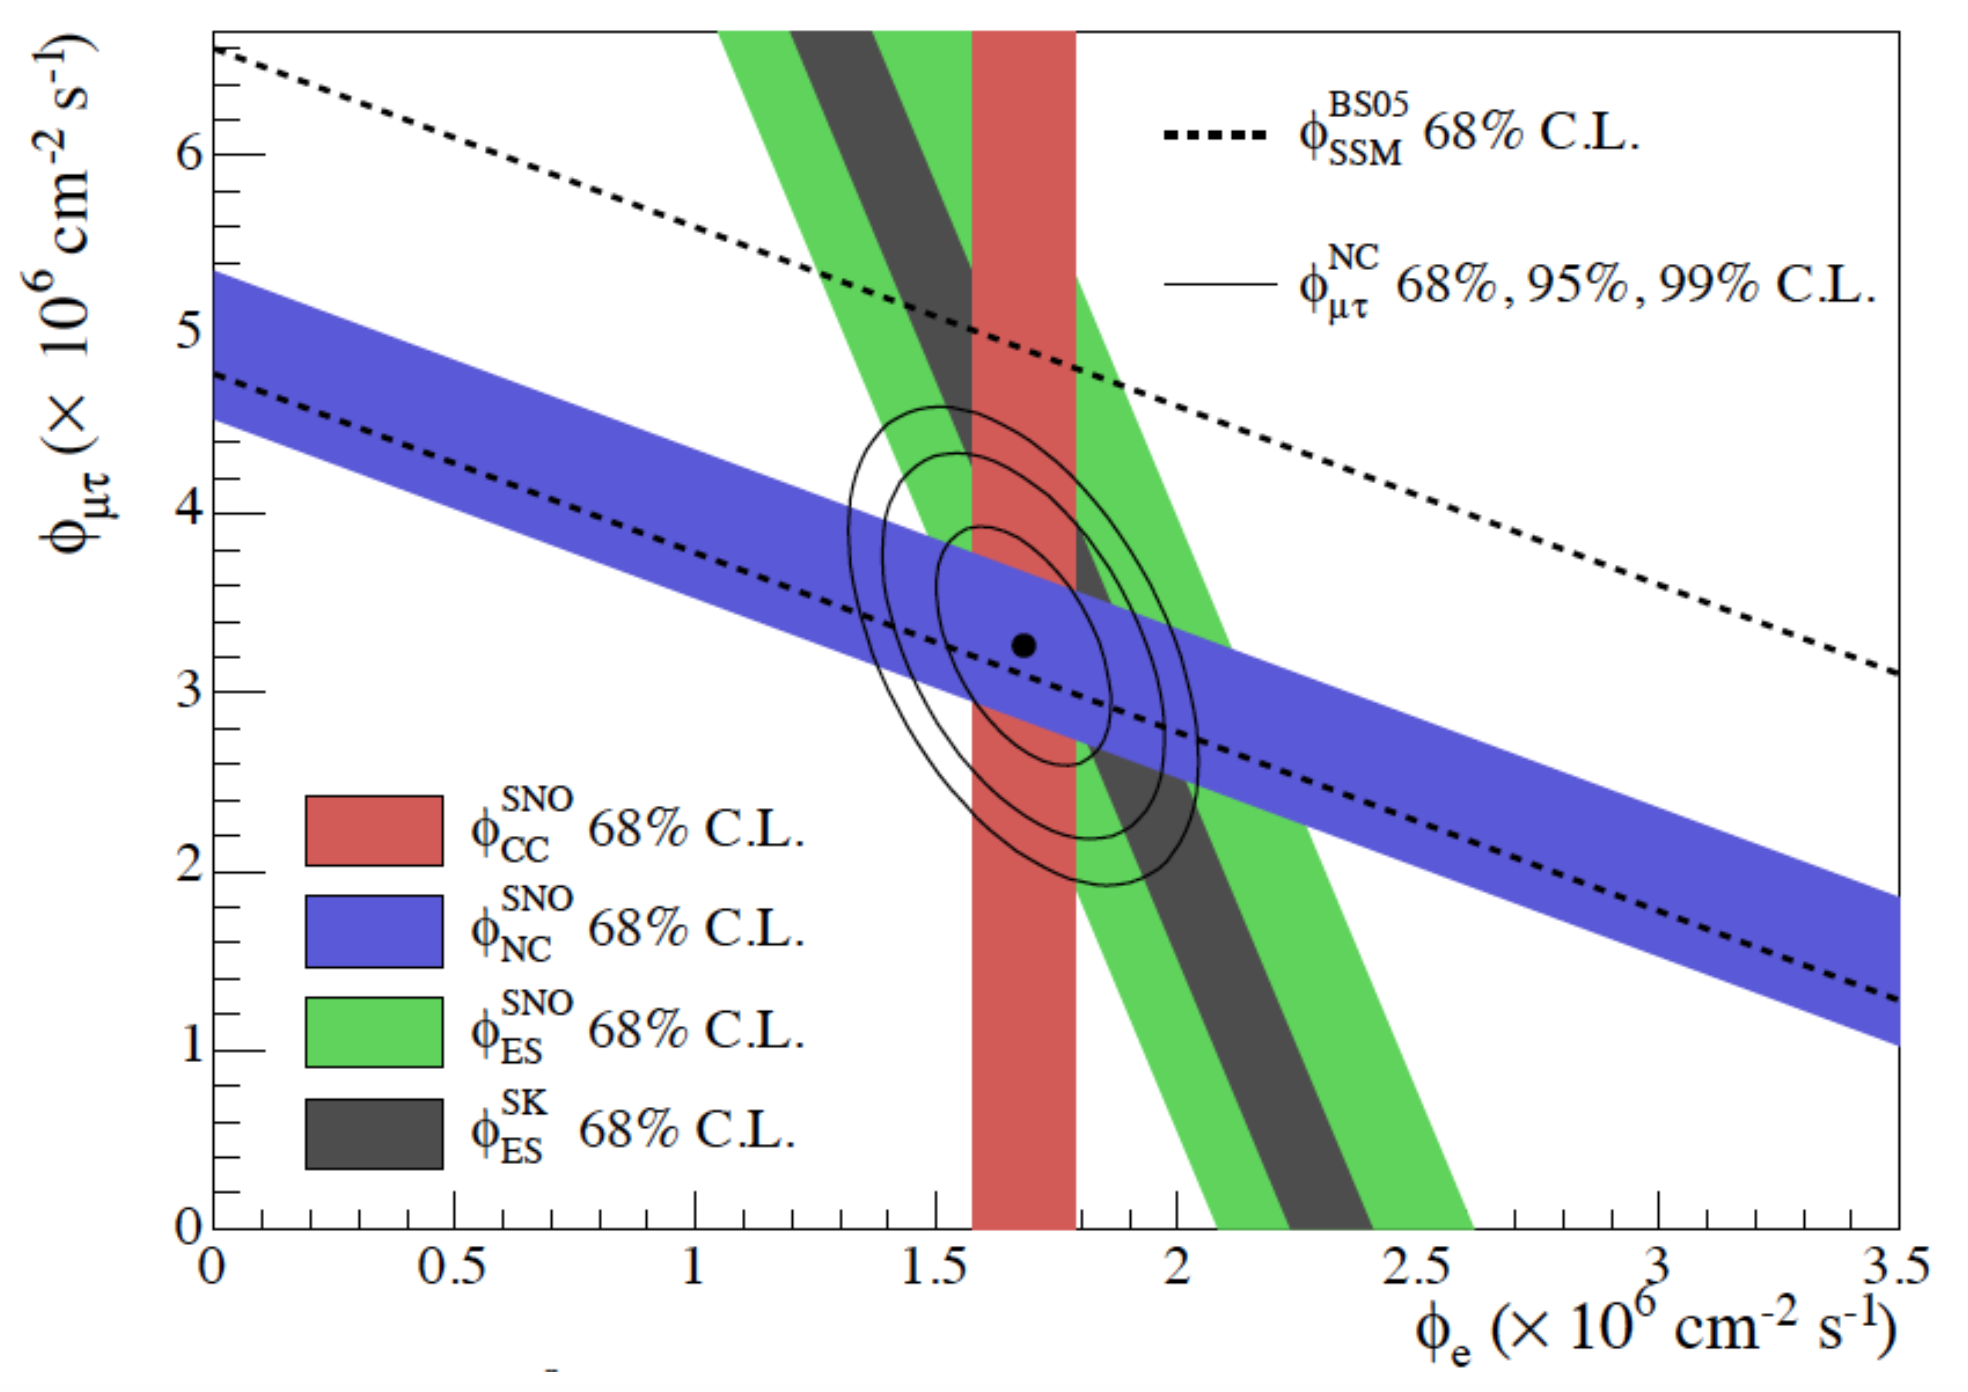
\includegraphics[width=\linewidth]{sno}
    \caption{The comparison of the fluxes $\nu_e$ and $\nu_{\mu,\tau}$ based on the measurements by SNO and Super-Kamiokande.}
    \label{fig:intro:sno}
  \end{minipage}
  \begin{minipage}{0.09\linewidth}
    \hspace{\linewidth}
  \end{minipage}
  \begin{minipage}{0.45\linewidth}
  \centering
    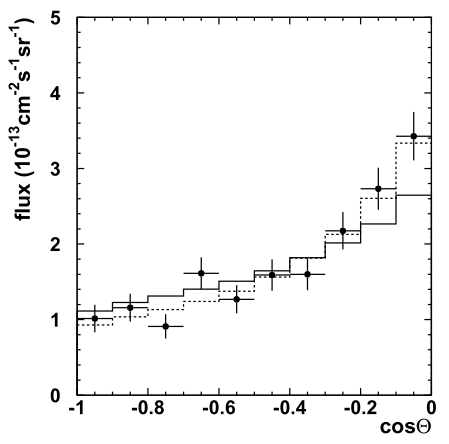
\includegraphics[width=\linewidth]{sk}
    \caption{The angular distribution of the muon and electron events in the Super-Kamiokande. The dotted histograms represented the simulation results w/o the neutrino oscillations and solid histograms corresponds to the best fit with oscillation hypothesis.}
    \label{fig:intro:sk}
  \end{minipage}
\end{figure}

But even after such brilliant confirmations of the phenomena the proof of the effect with the well-known source was essential. Such confirmation came with the measurements of the reactor antineutrinos with the KamLAND experiment~\cite{Eguchi2003}. It was the final confirmation of the neutrino oscillation phenomena.

\begin{figure}
  \centering
  \begin{minipage}{0.45\linewidth}
  \centering
    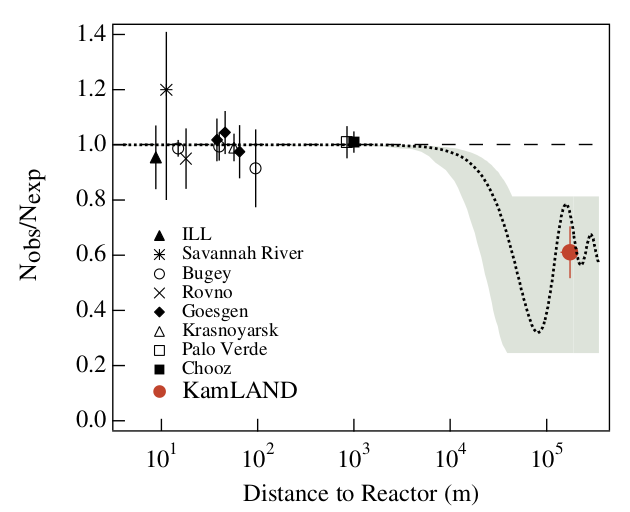
\includegraphics[width=\linewidth]{kam1}
    \caption{The ratio of the observed and expected neutrino flux from reactors. Figure from~\cite{Eguchi2003}.}
    \label{fig:intro:kam1}
  \end{minipage}
  \begin{minipage}{0.09\linewidth}
    \hspace{\linewidth}
  \end{minipage}
  \begin{minipage}{0.45\linewidth}
  \centering
    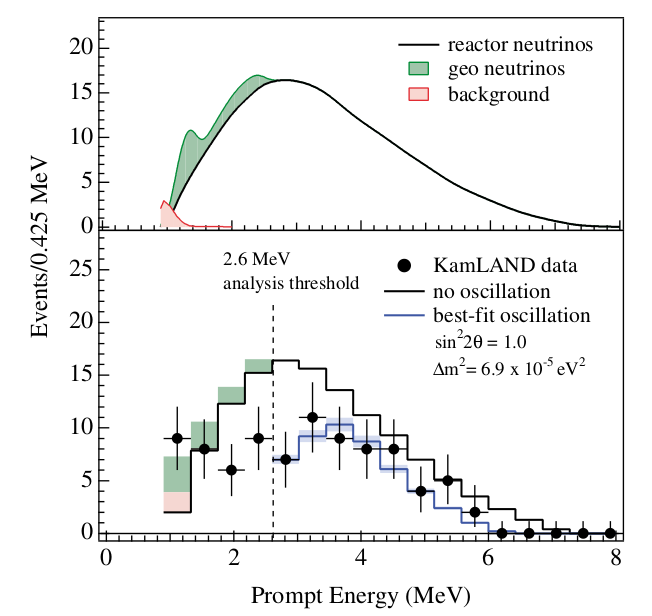
\includegraphics[width=\linewidth]{kam2}
    \caption{The energy spectrum of the neutrinos observed in the KamLAND experiment comparing to the expectations w/o neutrino oscillations. Figure from~\cite{Eguchi2003}.}
    \label{fig:intro:kam2}
  \end{minipage}
\end{figure}

\subsubsection{Modern experimental results}
After the discovery of the neutrino oscillations, many experiments study the phenomenon with different techniques.
\begin{itemize}
  \item Solar neutrinos: experiments Borexino, Super-Kamiokande. These experiments are powerful in $\theta_{12}$ angle constraints and can also measure $\Delta m_{21}^2$ and $\theta_{13}$
  \item Reactor experiments: KamLAND~\cite{Eguchi2003}, RENO~\cite{Ahn2012}, Double Chooz~\cite{Abe2014}, Daya Bay~\cite{An2014}. These experiments study the electron anti-neutrino disappearance and are sensitive to the  $\theta_{12}$, $\Delta m_{21}^2$ (KamLAND) and $\theta_{13}$, $\Delta m_{32}^2$ (RENO, Double Chooz, Daya Bay).
  \item Accelerator experiments: K2K~\cite{Ahn2006}, MINOS~\cite{Adamson2014}, T2K~\cite{Abe2020a}, NOvA~\cite{Acero2019}. These experiments started with studying muon (anti-)neutrino disappearance and MINOS, T2K and NOvA managed to observe the electron neutrino appearance, OPERA observed the tau neutrino appearance~\cite{Agafonova2014}. Thus these experiments are very precise in measurements of the $\theta_{23}$ angle and sensitive to the CP--violation. They can also measure $\theta_{13}$ and $\Delta m^2_{32}$ parameters
  \item Atmospheric and cosmology neutrinos: Super-Kamiokande~\cite{Jiang2019}, IceCube~\cite{Deyoung2005}. They can probe interesting processes in cosmology and also measure $\theta_{23}$, $\theta_{13}$, $\Delta m^2_{32}$ and $\delta_{CP}$ parameters, but less precisely comparing to the experiments mentioned above
\end{itemize}

So far the neutrino oscillation parameters are measured very precisely (\autoref{tbl:intro:osc}), but there is still room for the improvements.

\begin{table}[!ht]
\centering
  \begin{tabular}{||l|ll||ll|}
  \hline
  & \multicolumn{2}{c}{Normal Order} & \multicolumn{2}{c}{Inverse Order} \\
  \hline
  param                                   & best fit value  & 3$\sigma$range    & best fit value  & 3$\sigma$range \\
  \hline
  $\frac{\sin^2\theta_{12}}{10^{-1}}$     & 3.20            & 2.73$\to$3.79     & 3.20            & 2.73$\to$3.79 \\
  $\theta_{12}/^\circ$                    & 34.5            & 31.5$\to$38.0     & 34.5            & 31.5$\to$38.0 \\
  $\frac{\sin^2\theta_{23}}{10^{-1}}$     & 5.47            & 4.45$\to$5.99     & 5.51            & 4.53$\to$5.98 \\
  $\theta_{23}/^\circ$                    & 47.7            & 41.8$\to$50.7     & 47.9            & 42.3$\to$50.7 \\
  $\frac{\sin^2\theta_{13}}{10^{-2}}$     & 2.160           & 1.96$\to$2.41     & 2.220           & 1.99$\to$2.44 \\
  $\theta_{13}/^\circ$                    & 8.45            & 8.0$\to$8.9       & 8.53            & 8.1$\to$9.0 \\
  $\delta_{CP}/^\circ$                    & 218             & 157$\to$349       & 281             & 202$\to$349 \\
  $\frac{\delta m_{21}^2}{10^{-5}eV^2}$   & 7.55            & 7.05$\to$8.24     & 7.55            & 7.05$\to$8.24 \\
  $\frac{\delta m_{32}^2}{10^{-3}eV^2}$   & 2.42            & 2.334$\to$8.24    & -2.50           & -2.59$\to$-2.39 \\
  \hline

  \end{tabular}
  \caption{Summary of the neutrino oscillation parameters measurements from~\cite{Tanabashi2018} for both normal and inverse neutrino mass order.}
  \label{tbl:intro:osc}
\end{table}

The visual representation of the neutrino oscillation parameters constrains is presented in \autoref{fig:intro:osc_tot}.

\begin{figure}
  \centering
  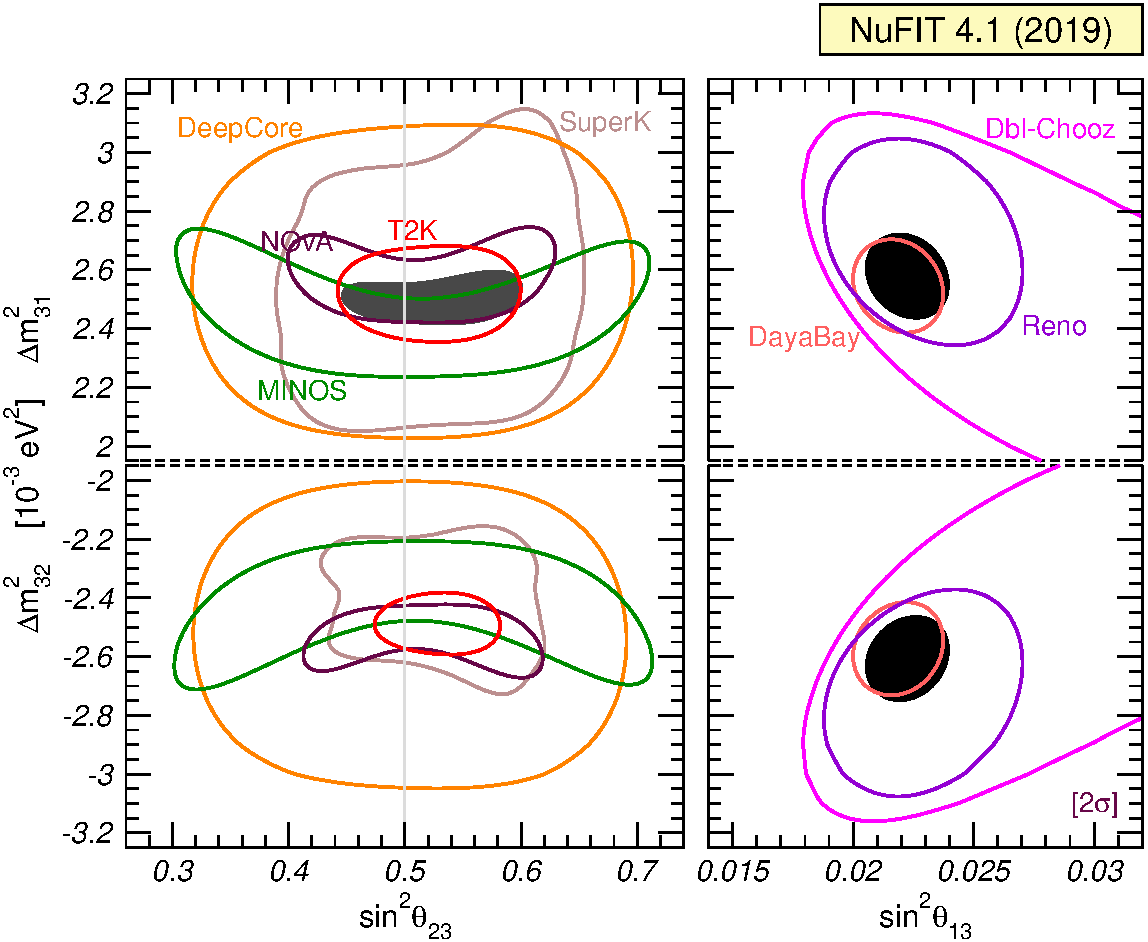
\includegraphics[width=0.8\linewidth]{osc_tot}
  \caption{The global fit of the neutrino oscillation parameters and results from the particular experiments used in the fit. The upper figures corresponds to the normal mass order and lower figures for inverted mass order. The figure from~\cite{Esteban2019}.}
  \label{fig:intro:osc_tot}
\end{figure}

The effect of the CP--violation is a subject of research nowadays. The accelerator experiments are more sensitive to this phenomenon. Both T2K and NOvA put their limits on the possible $\delta_{CP}$ values. The constraints are presented in \autoref{fig:intro:cp_fig}. The most recent T2K results providing 3$\sigma$ confidence interval on the $\delta_{CP}$ value are published in~\cite{Abe2020n}.

\begin{figure}
  \centering
  \begin{minipage}{0.49\linewidth}
    \centering
    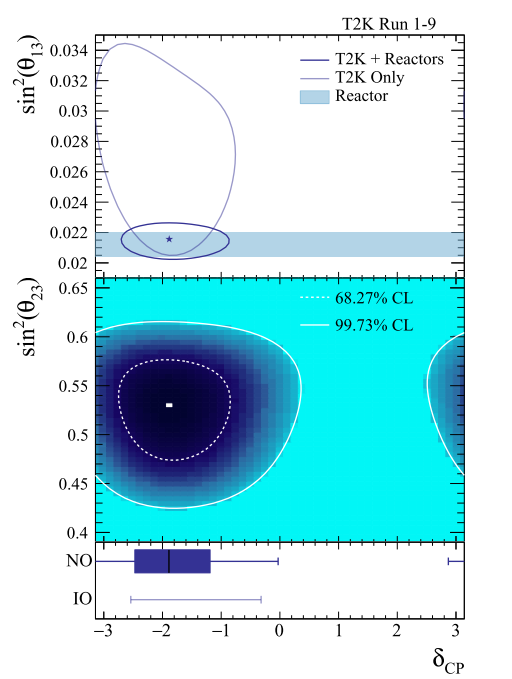
\includegraphics[width=\linewidth]{t2k_cp_const} \\ (a)
  \end{minipage}
  \begin{minipage}{0.49\linewidth}
    \centering
    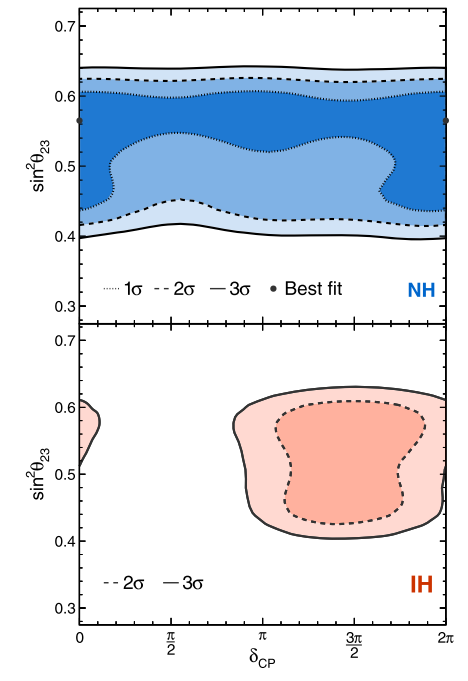
\includegraphics[width=\linewidth]{nova_cp} \\ (b)
  \end{minipage}
  \caption{Recent results of the CP--violation phase constraints in the T2K experiment (a)\cite{Abe2020n} and NOvA experiment (b)\cite{Acero2019}.}
  \label{fig:intro:cp_fig}

\end{figure}


\chapter{Neutrino mass}
\label{ch:intro:HNL}

As presented in the \autoref{sec:intro:osc} of \autoref{ch:nu_phys} the existence of the neutrino oscillation phenomenon explicitly indicates a non-zero mass difference between neutrino eigenstates. Thus at least two of three eigenstates should be massive. In the Standard Model of particle physics neutrinos are massless (\autoref{sec:sm} of  \autoref{ch:nu_phys}). A theory explaining the mass origin of the neutrino is required.

The easiest solution is to try to implement the same process which gives mass to all other particles in the SM --- Higgs mechanism~\cite{Higgs1964} (also called Englert-–Brout-–Higgs-–Guralnik-–Hagen-–Kibble mechanism for all contributed scientists). There are several problems in this approach:
\begin{itemize}
  \item the scale of the neutrino mass is very different from the other particles in the SM. The neutrino masses are less than 1 eV~\cite{Aker2019}, while the other particles masses are $m\gtrsim 0.5$ MeV, which gives a difference of at least 6 orders of magnitude. It can be even larger up to 8 orders in the case of minimum possible neutrino mass. It is hard to believe that the same mechanism is responsible for the generation of mass at so different scales.
  \item as described in the \autoref{sec:sm} only left-handed neutrinos and right-handed anti-neutrinos were observed. However for the Higgs mechanism both left and right-handed particles are required.
\end{itemize}

That leads to the fact that we need to implement some new mechanisms or/and new fundamental particles to explain the origin of the neutrino masses.

\section{Theory}
In this section, the main models of neutrino mass generation will be overviewed. The first idea is to describe the neutrino mass in the same way as masses of other fermions --- with Higgs mechanism. All the other fermions are described as a solution of the Dirac equation, thus referred to as a Dirac fermions. In the general solution of this equation a particle is different from its anti-particle. But in this assumption for the neutrino, the problem of the neutrino helicity rises. Since only left-handed neutrinos have been observed, but the theoretical framework requires both left and right-handed particles.

Another approach is to use a specific solution of the Dirac equation. Majorana proposed the fermion that is invariant under particle/anti--particle symmetry. Neutrino is the only candidate to be such a particle as it is the only neutral fundamental fermion. This theory gives an interesting opportunity to describe the neutrino mass and also open the door for the new physics beyond the Standard Model.

However, the most interesting hypothesis is mixing Dirac and Majorana theories. An example of such a hypothesis is a ``see--saw'' mechanism. It provides a natural explanation of the tiny neutrino mass through the mixing with the heavier partner. The Higgs mechanism is used at the same scale as in the SM (~GeV) and new physics beyond the SM is implemented. Nevertheless, the new exotics particles appear only at the extremely large energy scale. That explains why they have not been observed.

\subsection{Dirac mass term}
In the Standard Model of particle physics, the masses of all the particles are generated with the Higgs mechanism. The Higgs-lepton Yukawa Lagrangian provides an explanation for the masses for the charged leptons
\begin{equation}
\mathcal{L}_{H, L}=-\sum_{\alpha, \beta=e,\mu,\tau}Y'^\ell_{\alpha\beta}\overline{L'_{\alpha L}}\Phi\ell'_{\beta R}+h.c
\end{equation}
Applying the same approach for the neutrino mass generation we will get the Lagrangian
\begin{align}
\mathcal{L}&=-\sum_{\alpha\beta=e,\mu,\tau}\bar{\nu}_{L,\alpha}(m_D)_{\alpha\beta}\nu_{R,\beta}+h.c. =\nonumber \\
&=-\overline{\nu_L}m_D\nu_R+h.c.
\end{align}
where $m_D$ is a 3x3 complex matrix, corresponding to 3 neutrino generations, $\nu_L$ and $\nu_R$ are a left--handed and right--handed neutrino. It can be diagonalized $m_D=U^\dag m V$, where U and V are unitary and $m_i\delta_{ik}$, $m_i>0$. After diagonalization, we can separate

\begin{align}
\nu_{\alpha L}&=\sum_iU_{\alpha i}\nu_{iL} \nonumber \\
\nu_{\alpha R}&=\sum_iV_{\alpha i}\nu_{iR}
\end{align}
and define $\nu\equiv\nu_L+\nu_R$. Thus the Dirac mass term will be expressed as
\begin{equation}
\label{eq:intro:dirac}
\mathcal{L}^{D}_{mass}=-\sum_im_i\overline{\nu_i}\nu_i
\end{equation}
where $\nu_i$, $i=1, 2, 3$ are neutrino mass eigenstates and $\nu_{\alpha L}$ are left-handed neutrino flavor eigenstate. Their mixing is defined with PMNS matrix (\autoref{eq:intro:mixing}). The equations above implement the right-handed neutrino $\nu_R$ that is essential for the Higgs mechanism, but has not been observed in the experiments. It happens because the weak interaction allows only left-handed neutrino to interact with matter.

\subsection{Majorana mass term}
The Dirac fermion is the most general solution of the Dirac equation. But there is an interesting particular solution. A Majorana fermion satisfies Dirac equation under the assumption that this particle is the same as its anti--particle ($\psi=\psi^C$). Neutrino is the only candidate to be a Majorana fermion as it is the only neutral fundamental fermion. The charged fermion obviously can not satisfy such a condition because particle and anti--particle carry an opposite electric charge. Whether neutrino is a Majorana fermion is still an open question, but such a hypothesis provides interesting consequences. To generate the mass for such a particle we need only one chiral fermion field. As neutrino is left-handed let us denote is as $\nu_L$. To write the mass term for this specific case we need to use $\nu_L$ alone. Modifying \autoref{eq:intro:dirac}
\begin{equation}
\mathcal{L}^D_{mass}=-m\overline{\nu}\nu=-m\left(\overline{\nu_R}\nu_L+\overline{\nu_L}\nu_R\right)=-m\overline{\nu_R}\nu_L+h.c.
\end{equation}

Here $\nu_R$ should be replaced with the right-handed function of the $\nu_L$. It is the charge conjugated field
\begin{equation}
\nu_L^C=\mathcal{C}\overline{\nu_L}^T
\end{equation}
Thus the Majorana mass term can be expressed as
\begin{equation}
\mathcal{L}^M_{mass}=-\frac{1}{2}m\overline{\nu_L^C}\nu_L+h.c.
\end{equation}

The Majorana mass term provides an interesting mechanism for the generation of the neutrino mass. But it implements also physics beyond the SM. The lepton number is invariant in the SM because of a global U(1) symmetry. With the Majorana model, there is no such symmetry anymore. This leads to the processes where the lepton number is violated, e.g. neutrino-less double beta decay.


\subsection{Mixing Dirac and Majorana terms}
The most interesting approach is a combination of both Dirac and Majorana terms. In this case, the model is very flexible and can provide an explanation of the neutrino masses with minimum extension of the Standard Model. The mass term will be written with
\begin{equation}
\label{eq:intro:comb}
\mathcal{L}_{mass}^{D+M}=\mathcal{L}^D_{mass}+\mathcal{L}^R_{mass}+\mathcal{L}^L_{mass}
\end{equation}
where
\begin{align}
\mathcal{L}^L_{mass}&=\frac{1}{2}\sum_{\alpha,\beta}\nu'^T_{\alpha L}\mathcal{C}^\dagger M^L_{\alpha\beta}\nu'_{\beta L}+h.c. \\
\mathcal{L}^R_{mass}&=\frac{1}{2}\sum_{s, s'}\nu^T_{s R}\mathcal{C}^\dagger M^R_{ss'}\nu'_{s' R}+h.c. \\
\mathcal{L}^D_{mass}&=-\sum_{s=s_1, ..., s_{N_s}}\sum{\alpha}\overline{\nu}_{sR}M^D_{ss'}\nu'_{\alpha L} +h.c.
\end{align}

In the equations above the Greek indexes, as usual, corresponds to the flavor states, L and R illustrate the chirality and $s_i$ describes the sterile neutrino types. Thus the matrix $M^L$ will be symmetric 3x3, $M^R$ --- symmetric $N_s\times N_s$ and $M^D$ --- $N_s\times3$. The mass matrix for combination of these three components will be written with
\begin{equation}
M^{D+M}\equiv
\begin{pmatrix}
M^L & {M^D}^T \\
M^D & M^R
\end{pmatrix}
\end{equation}

The mass states will be given by

\begin{align}
\nu_R^C\equiv
\begin{pmatrix}
\nu^C_{s_1R} \\
\vdots \\
\nu^C_{s_{N_S}R}
\end{pmatrix}
&&
N'_L\equiv
\begin{pmatrix}
\nu'_L \\ \nu^C_R
\end{pmatrix}
\end{align}

And the mass term \autoref{eq:intro:comb} with new notations will be rewritten as
\begin{equation}
\mathcal{L}_{mass}^{D+M}=\frac{1}{2}N'^T\mathcal{C}^\dagger M^{D+M}N'_L+h.c.
\end{equation}

There are different ways to combine Dirac and Majorana terms. With different initial assumptions, the theory result can be quite different. Here there are the main hypotheses. The notation $m_D$ describes the Dirac mass, $m_L$, $m_R$ describe Majorana mass and the $m_{1,2}$ describes the mass eigenstates observable in the experiment.
\begin{itemize}
  \item Maximal mixing. $m_L=m_R$, $m_{2, 1}=m_L\pm m_D$, $\Delta m^2=m_2^2-m_1^2=4m_L m_D$
  \item Dirac limit. $m_L=m_R=0$, $m_{2,1}=\pm m_D$
  \item Pseudo-Dirac neutrinos. $\left|m_L\right|,m_R \ll m_D$, $m_{2,1}\approx\frac{m_L+m_R}{2}\pm m_D$
  \item See--saw mechanism. $m_D \ll m_R$, $m_L=0$
\end{itemize}

\subsubsection{See--saw mechanism}
Among all of the theories with Dirac and Majorana mixing the see--saw mechanism seems to be the most promising. Here are the main advantages of this hypothesis:
\begin{itemize}
  \item The gauge symmetry is not broken as $m_L=0$
  \item The only ``exotic'' part (SM extension) is the implementation of $m_R$
  \item The Dirac mass can be easily explained with the Higgs method as $m_D$ is close to the mass of the SM particles
  \item Tiny mass of the observed neutrino eigenstates is understood as $m_D$ is scaled with $m_R$
\end{itemize}

So, how can we explain the fact that observed neutrino mass is so small? $m_D$ is generated with a Higgs mechanism and can be at the GeV scale. $m_R$ is an exotic part of the theory. As it is a Majorana term it will violate the lepton number. But it will take place only at extremely high energies, much higher than the electroweak scale. The observed neutrino mass at first order will be given by the mixing:
\begin{align}
m_1\approx\frac{m_D^2}{m_R} \ll m_D && m_2\approx m_R \gg m_D
\end{align}

and the mixing angle will be given by

\begin{equation}
\theta\approx\frac{m_D}{m_R} \ll 1
\end{equation}

For example, imagine the Dirac mass is fixed at $m_D=170 GeV$ and observed neutrino mass $m_1=5\times 10^{-2} eV$, then the Majorana mass will be at an extremely high energy scale $M_R\approx10^{15}GeV$.

\subsection{Heavy Neutral Lepton}
\label{sec:intro:HNL}
In the previous section, it was proven that an extension of the SM is necessary to explain the neutrino mass. The see--saw mechanism is a minimal extension that can provide such an explanation. But there is no hint for the mass scale of the proposed new particles.

\subsubsection{Light sterile neutrino}
The special case is the light sterile neutrino with $m\approx1eV$. To meet the agreement with the LEP results of the Z boson decay measurements (\autoref{sec:intro:LEP}) the 4th neutrino should not couple with the Z boson. That's why such a particle is notated as a ``sterile'' neutrino. Also, their mixing with the other three active neutrinos should be quite small $\left|U_{e4},\right|, \left|U_{\mu4},\right|, \left|U_{\tau4},\right| \ll \left|U_{s4},\right|$. In most of the neutrino oscillation experiments 3-flavor neutrino model describes the observation quite well. However, in some experiments, an anomaly that can be explained with the 4th neutrino with $\Delta m_{41}^2\approx1eV$ was found. The first such an experiment was LSND~\cite{Athanassopoulos1997}, followed by MiniBooNE~\cite{Aguilar-Arevalo2010}, that inspired the short-baseline neutrino oscillation research program. Some anomalies have also been found in the experiments with neutrinos from reactors and with solar neutrinos in the gallium experiments. However, there is no final conclusion if it is a significant observation or the result of the unaccounted systematic error. Many experiments are running now in order to figure out the nature of the phenomenon. We can generally divide them in the short-baseline accelerator experiments: MicroBooNE, Short Baseline Program in Fermilab, and others, and reactor experiments: NEOS~\cite{Ko2017}, DANSS~\cite{Alekseev2018}, STEREO~\cite{Almazan2018}, PROSPECT~\cite{Ashenfelter2018}, NEUTRINO-4~\cite{Serebrov2015}, SoLid, and others.

More information about the light sterile neutrino can be found in~\cite{Abazajian2012}.

\subsubsection{Neutrino Minimal Standard Model ($\nu MSM$)}
\label{sec:intro:numsm}
A minimal extension of the SM introducing the neutrino mass explanation was developed by Asaka and Shaposhnikov~\cite{Asaka2005}. The existence of three heavy neutrinos $N_1$, $N_2$, $N_3$ was proposed. It is worth mentioning that there are several extensions of the SM with different numbers of additional particles. $\nu MSM$ is highlighted because of its minimalism, which has always been an advantage of the physics theory.

Long living (comparing to the Universe's age) $N_1$ with a mass around keV can be responsible for the phenomenon of the Dark Matter. It can be produced in the early Universe and can still exist. $N_1$ can explain the gravitational anomalies such as galaxies mass and galaxy rotation speed.

$N_2$ and $N_3$ are two nearly degenerated fermions with masses in the range $140 MeV < M < 80 GeV$. The model contains 6 CP-violating phases that allow the violation of the lepton number $L$. Such an asymmetry can be transferred to the active leptons through the mixing with the active neutrino. With the help of the sphaleron mechanism, the violation of the lepton number can cause the violation of the baryon number $B$, but conserving the $B-L$. Hence the model can explain the observed baryon asymmetry of the Universe~\cite{Asaka2005a}.

\section{Experiments}
Despite the Standard Model assumption about the massless neutrino nature, there were several attempts to measure its mass. After the confirmation of the fact that neutrino has mass from the neutrino oscillation phenomenon (\autoref{sec:intro:osc}), these measurements became essential.

\subsection{Neutrino mass measurements}
In this section, both direct and indirect methods of the neutrino mass measurements will be overviewed. The latest experimental results will be presented.

\subsubsection{Beta decay}
The straightforward approach for the neutrino mass measurements is a search for the effect of the nonzero neutrino mass in the beta decay spectrum. One needs to measure the energy of outgoing electrons and look at the far end of the distribution. The variation of the neutrino mass changes dramatically the energy spectrum in this particular region. For the electron source, a deuterium or a tritium isotope is usually chosen. The main technological issues are to perform extremely precise measurements of the electron energy. The most accurate limits obtained with this method for a long time belonged to Mainz~\cite{Kraus2005} and Troitsk~\cite{Aseev2011} experiments. Recently KATRIN experiment announced more precise neutrino mass limits $m_\nu < 1.1 eV$ with 90\%C.L.~\cite{Aker2019}.

It is important to notice what is the ``neutrino mass'' $m_\nu$ that is measured in the beta decay. Because of the lepton mixing the mass eigenstates can not be measured independently, but only in the superposition.
\begin{equation}
m_\nu\equiv m_\beta\equiv\sqrt{\sum_i\left|U_{ei}\right|^2m_i^2}
\end{equation}

More details about the neutrino mixing were presented in \autoref{sec:intro:osc}.

\subsubsection{Neutrinoless double beta decay}
If the neutrino has a Majorana nature, it is possible to measure the $m_{\beta\beta}$ in the process of the neutrinoless double beta decay. The Feynman diagram of the process is shown in \autoref{fig:intro:bb}.
\begin{equation}
m_{\beta\beta}=\sum_i U^2_{ei}m_i
\end{equation}

\begin{figure}
  \centering
  \begin{minipage}{0.45\linewidth}
    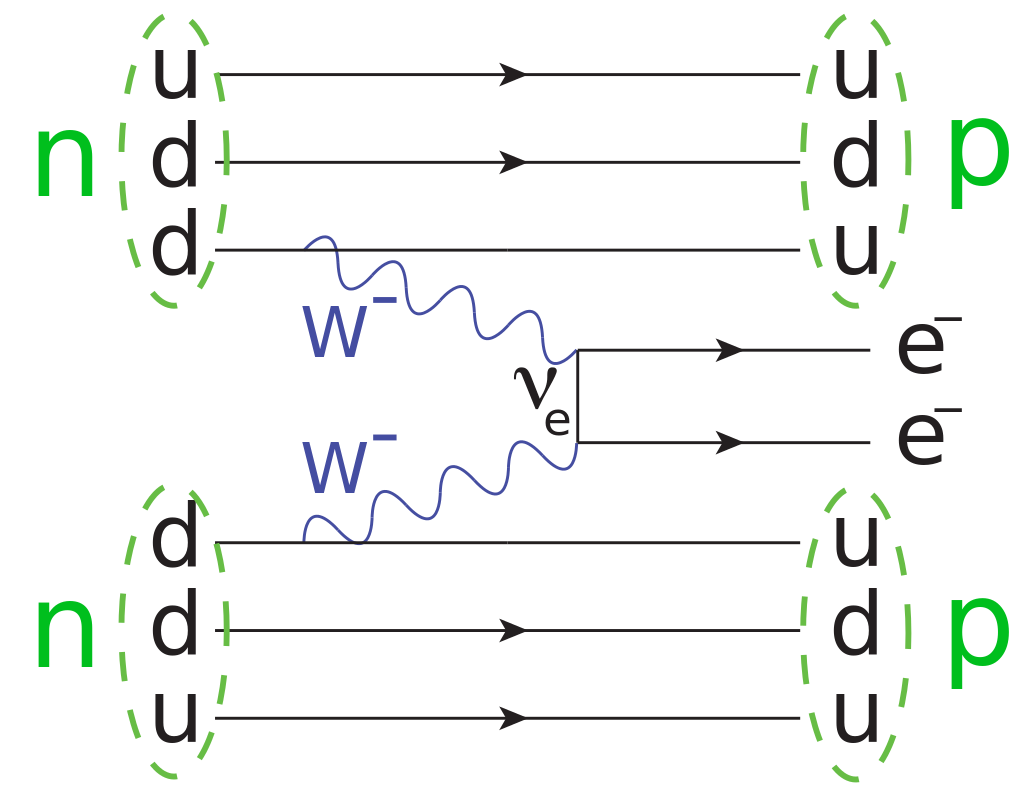
\includegraphics[width=\linewidth]{beta_beta}
    \caption{Feynman diagram for the neutrinoless double beta decay}
    \label{fig:intro:bb}
  \end{minipage}
  \begin{minipage}{0.09\linewidth}
  \end{minipage}
  \begin{minipage}{0.45\linewidth}
    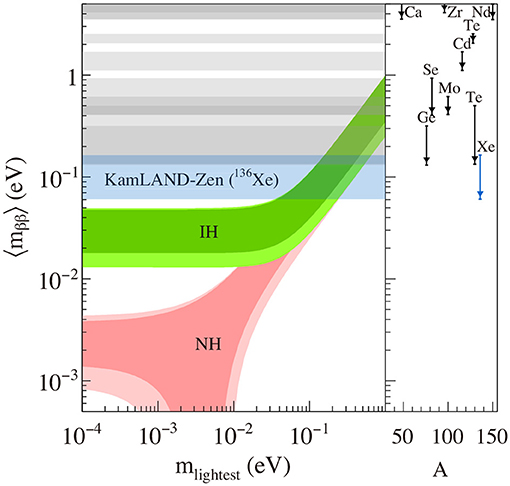
\includegraphics[width=\linewidth]{beta_beta_limit}
    \caption{The current limits on the $m_{\beta\beta}$ and the allowed regions for both normal and inverse mass ordering.}
    \label{fig:intro:bb_lim}
  \end{minipage}
\end{figure}

All the $0\nu\beta\beta$ experiments are putting the limits on the $m_{\beta\beta}$ value. The most precise result was obtained by KamLAND-Zen experiment $m_{\beta\beta} < (61-165) meV$ 90\% C.L.~\cite{Gando2016}. Relatively large uncertainties comes from the poor knowledge about nuclear matrix elements. The summary of all the constraints from different experiments is shown in \autoref{fig:intro:bb_lim}. One should keep in mind that successful measurement is possible only in the case of Majorana neutrino nature.

\subsubsection{Cosmology}
Cosmology provides different possibilities for neutrino mass measurements. One of the earliest attempts was done based on the timing measurements of the neutrinos from SN1987 --- the earliest and so far the only observation of the neutrino from the supernova collapse.

The other method is a precise observation of the evolution of the early Universe. The combination of the cosmic microwave background (CMB) and baryon acoustic oscillation provides the limit on the neutrino mass $m_\nu=\sum_i m_{\nu_i}<0.12eV$ 90\% C.L.~\cite{Palanque-Delabrouille2015}.

The main problem of such analyses is a dependence on the theoretical models such as supernova collapse or early Universe evolution.

\subsection{Search for Heavy Neutral Lepton}
\label{sec:intro:HNL_exp}
As mentioned in the \autoref{sec:intro:HNL}, there are several models proposing the existence of the Heavy Neutral Lepton (HNL). Various analyses in different experiments were performed to find the HNL. In this section, we will describe the search for the HNL in the context of the $\nu MSM$ framework, but the results can be applied for other models introducing the heavy neutrino via mixing with the active one.

\subsubsection{HNL at keV scale}
The lightest HNL at the keV scale can be detected through its decays $N_1\to \nu\nu\overline{\nu}$ and $N_1\to\gamma\nu$. While the first reaction is undetectable from the practical point of view, the latter will produce the observable X-rays. There are several analyses searching for the X-ray signal from the cosmological object (e.g. Galaxy core, other galaxies, etc.)~\cite{Ng2019, Perez2017}. The latest results are presented in \autoref{fig:intro:hnl_kev}.

\begin{figure}[!ht]
  \centering
  \begin{minipage}{0.49\linewidth}
    \centering
    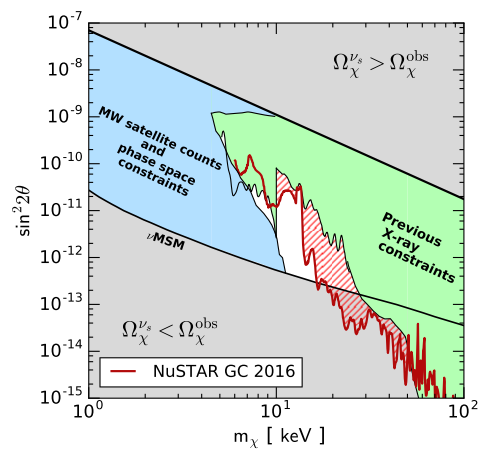
\includegraphics[width=\linewidth]{kev_gen} \\ (a)
  \end{minipage}
  \begin{minipage}{0.49\linewidth}
    \centering
    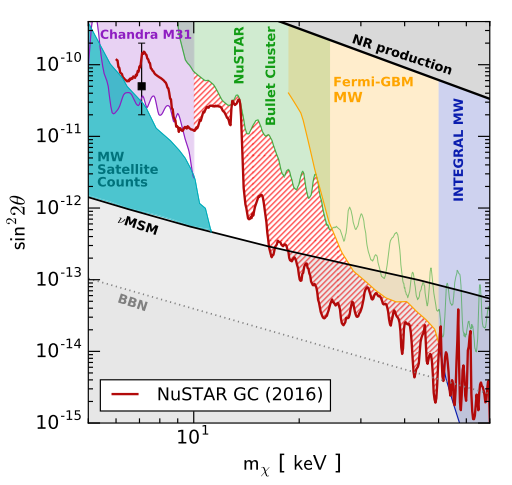
\includegraphics[width=\linewidth]{kev_det} \\ (b)
  \end{minipage}
  \caption{The constrains on the mixing angle of the $N_1$ with respect to its mass: (a) the general figure and (b) the detailed view at the region of interest. Figure provided by~\cite{Perez2017}.}
  \label{fig:intro:hnl_kev}
\end{figure}

So far the region is almost excluded but there is still a possibility to find $N_1$ from $\nu MSM$~\cite{Caputo2020}.

\subsubsection{HNL at GeV scale}
This is a scale where we expect to find the heavy neutrinos $N_2$ and $N_3$ from the $\nu MSM$. Its mass allowed the direct search through the decay into SM particles. The work~\cite{Gorbunov2007} provides a detailed overview of the HNL production and the decay modes. The main production mode is a meson two-body decay.
\begin{equation}
H\to\ell+N
\end{equation}
Thus we can expect the HNL production in the decays of $\pi$, $K$, $D$, $B$ and heavier mesons. The HNL is unstable hence the decay channel into the active lepton is open. The decay modes to the lighter HNL $N_{1,2}\to N_1+...$ are strongly suppressed. Thus the most probable modes are
\begin{equation}
N\to\overline{\nu}\nu\nu,\text{   } \mu e\nu, \text{   }\pi^0\nu, \text{   }\pi e, \text{   }\mu\mu\nu, \text{   }\pi\mu, \text{   }Ke,\text{   } K\mu,\text{   } \eta\nu, \text{   }\rho\nu,...
\end{equation}

The two-body decay modes are more probable over the three-body decay modes, hence they are preferable for the direct search in the experiment. Also, the channels with at least two charged particles in the final state are much easier for the observation. Thus $3\nu$ and $\pi^0\nu$ modes are often not considered in the analysis due to an extremely hard detection.

In general, the HNL search can be separated into several categories:
\begin{itemize}
  \item analysis of the meson decay. The effect is proportional to $\left|U\right|^2$. For example, E949 and NA62 explored the decay $K^+\to\mu^+N$. Thus the region of the HNL mass $M_{HNL} < m_K-m_\mu=388 MeV/c^2$ can be explored.
  \item direct search for the HNL decay. For example, PS191 experiment searched for the HNL produced with $\pi/K\to eN$ and $\pi/K\to\mu N$ and further decayed into $e\pi$, $\mu\pi$, $\mu e\nu$.
  \item a direct search can be performed in the collider experiments. DELPHI and LHCb looked for the HNL decays, produced in the Z boson decay.
  \item joint search for HNL production and decay. For example, ATLAS and CMS performed the search for the two leptons with the same charge: one lepton along with HNL production the other comes from its decay. Such a process is possible only in the case of the Majorana nature of the HNL.
\end{itemize}

So far, no evidence of the HNL existence was found and upper limits on the mixing angles were set. The latest results from all the experiments can be found in \autoref{fig:umuh}, \autoref{fig:ueh} and \autoref{fig:utauh}.

\begin{figure}[!ht]
\centering
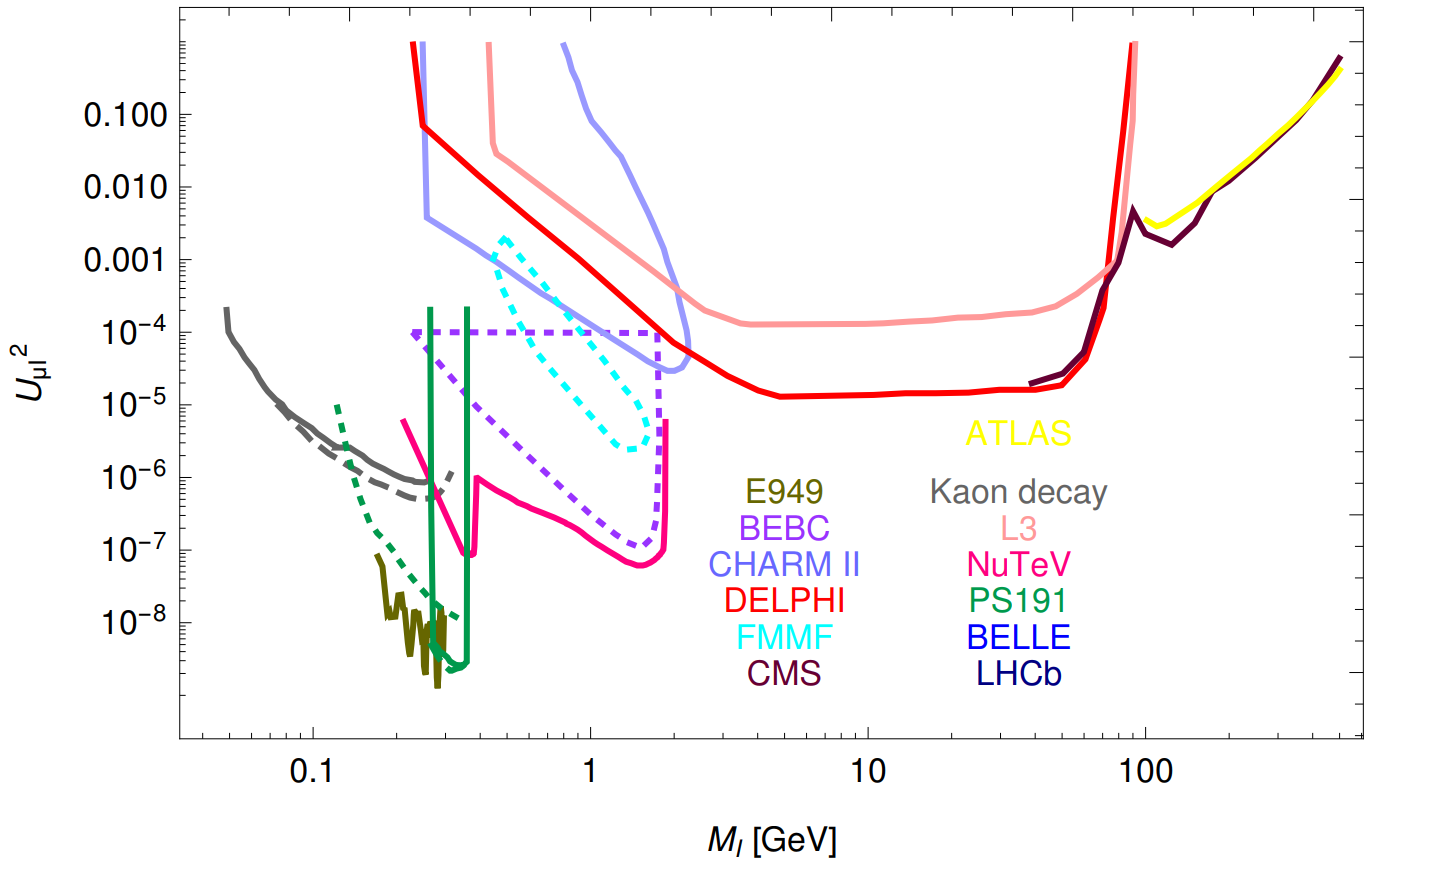
\includegraphics[width=0.7\linewidth]{umuh}
\caption{Constraints on the mixing matrix element $|U_{\mu}|^2$ from the experiments CMS~\cite{cms}, DELPHI~\cite{delphi}, L3~\cite{l3}, LHCb~\cite{lhcb}, BELLE~\cite{belle}, BEBC~\cite{bebc}, FMMF~\cite{fmmf}, E949~\cite{e949}, PIENU~\cite{pienu}, TRIUMF/TINA~\cite{triumf}, PS191~\cite{Bernardi1988}, CHARMII~\cite{charm2}, NuTeV~\cite{nutev}, NA3~\cite{na3} and kaon decays in~\cite{kaon2}. The plot is similar to Ref.~\cite{drewes}, some comments on the interpretation can be found in that article and references therein.}
\label{fig:umuh}
\end{figure}
\begin{figure}[!ht]
\centering
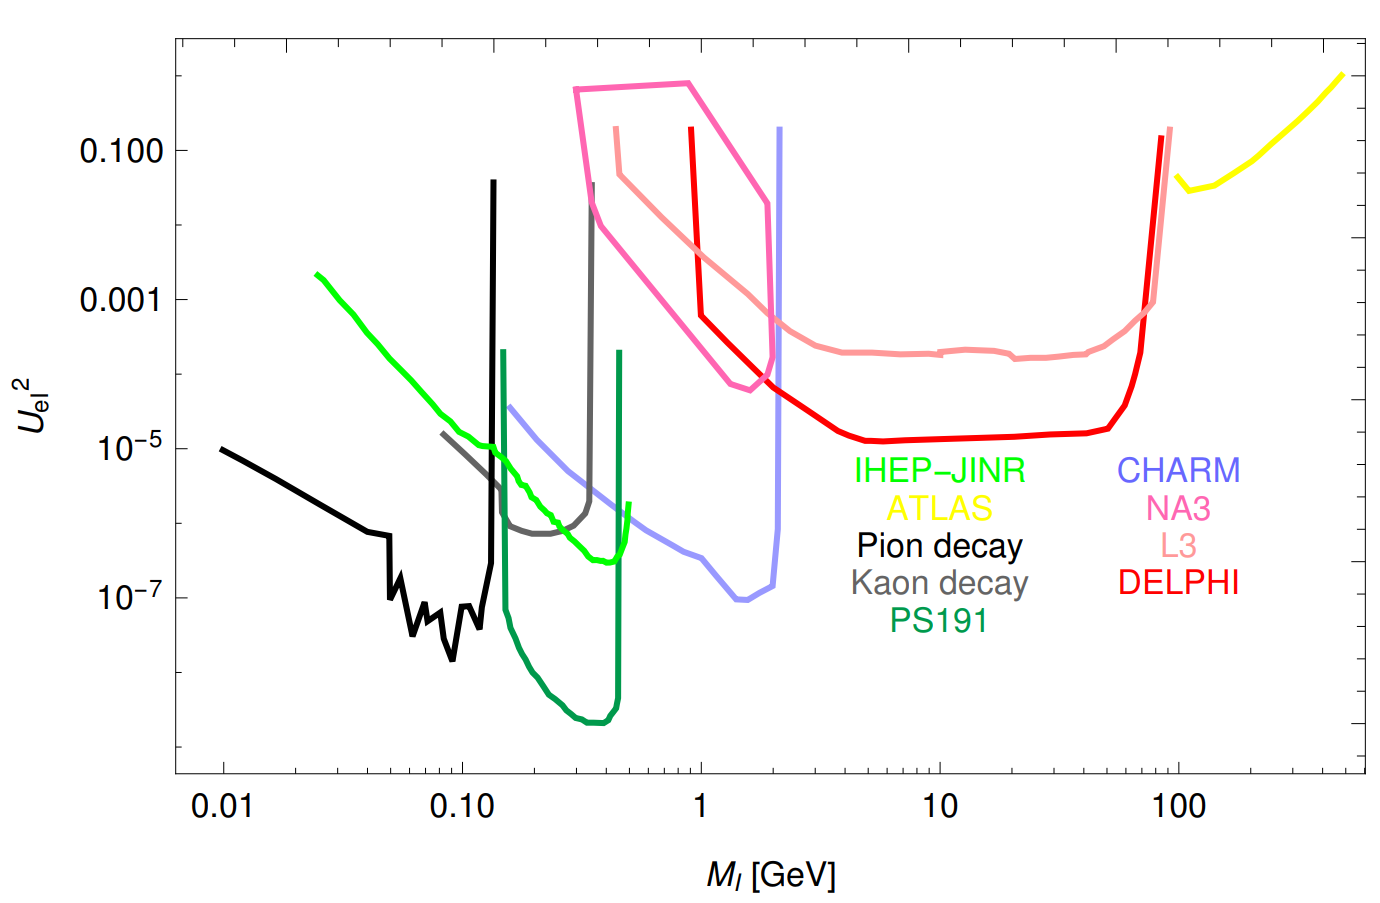
\includegraphics[width=0.7\linewidth]{ueh}
\caption{Constraints on the mixing matrix element $|U_{e}|^2$ from the experiments  DELPHI~\cite{delphi},  L3~\cite{l3}, PIENU~\cite{pienu}, TRIUMF/TINA~\cite{triumf}, PS191~\cite{Bernardi1988}, CHARM~\cite{charm}, NA3~\cite{na3}, IHEP-JINR~\cite{jinr} and kaon decays. The plot is similar to Ref.~\cite{drewes}, some comments on the interpretation can be found in that article and references therein.}
\label{fig:ueh}
\end{figure}
\begin{figure}[!ht]
\centering
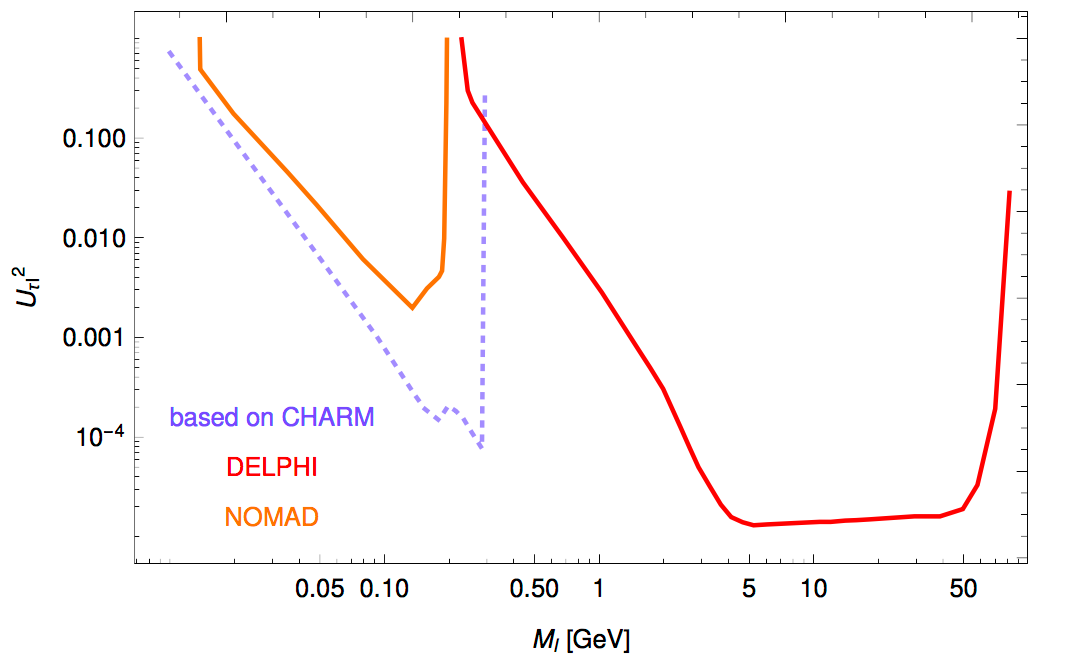
\includegraphics[width=0.7\linewidth]{utauh}
\caption{Constraints on the mixing matrix element $|U_{\tau}|^2$ from the experiments  CHARM~\cite{orloff2002limits}, NOMAD~\cite{baldisseris2001search}, DELPHI~\cite{delphi} and L3~\cite{l3}, some comments on the interpretation can be found in that article and references therein.}
\label{fig:utauh}
\end{figure}

\section{Prospects of the neutrino physics}
In the introduction part, it was highlighted several times that we still have several open questions in the neutrino physics. The most important among them are:
\begin{itemize}
  \item CP-violation in the lepton sector. Does it exist?
  \item Is neutrino a Dirac or a Majorana fermion?
  \item What is the neutrino mass order? $m_1<m_2<m_3$ or $m_3<m_1<m_2$?
  \item What are the absolute values of the neutrino mass?
  \item What is the nature of the neutrino masses?
  \item What are the other neutrinos except known 3 generations?
  \item Can neutrino (or heavy neutrino) solve the problems of modern cosmology: Dark Matter existence and the matter-dominance in the Universe?
\end{itemize}

Answer for any of them will be a remarkable step forward in our understanding of fundamental physics.

\section{Future neutrino experiments}
\label{intro:future}
Several experiments are working on solving the problems above. Many proposals were made about future experiments.

The ongoing long-baseline accelerator experiments T2K and NOvA already observed a hint for the maximal CP-violation in the neutrino oscillations. The T2K experiment will be able to reach $3\sigma$ sensitivity for some values of the $\delta_{CP}$~\cite{Abe2016e}. The future experiments Hyper-Kamiokande~\cite{Proto-Collaboration2018} and DUNE~\cite{Acciarri2016} are proposed to reach $5\sigma$ sensitivity for almost all the values of the $\delta_{CP}$.

The JUNO experiment~\cite{Cerna2020} is going to perform the extremely precise measurements of the reactor anti--neutrino oscillations. With the help of these observations the neutrino mass order can be determined.

Several experiments are looking for the neutrino-less double-beta decay. They are looking for small signal in the low background environment. Different isotopes are used as a supposed source of the $0\nu\beta\beta$ decay. KamLAND-ZEN uses the ${}^{136}Xe$ isotope, GERDA~\cite{DiMarco2020} uses ${}^{76}Ge$, CUORE~\cite{Cardani2020} ${}^{82}Se$ and SNO+ ${}^{130}Te$. Any of the positive results will indicate the Majorana nature of the neutrino.

Astrophysics experiments are studying neutrino from the sources outside of the Solar System. Usually, they are using Cherenkov light from the lepton or other particles produced in the neutrino interactions. The probability of such events is relatively low, so the fiducial volume is extended as much as possible. But the energy of such events is quite high. The examples of such experiments are IceCube~\cite{Aartsen2017} using 1 $km^3$ of ice at the South Pole; Antares --- the first sea neutrino telescope; proposed experiment KM3NeT~\cite{LeBreton2019} is a one cubic kilometer neutrino telescope in the Meridian sea. These experiments can detect the neutrinos from the supernova core or active galaxy core that makes them very powerful for testing the cosmological models.

The very important class of the experiments are searching for sterile neutrino in the reactor experiments. Some anomalies, e.g. lack of the neutrino events in the short-baseline reactor experiments or Gallium experiments can be explained with the implementation of the 4th neutrino flavor. The extremely short-baseline reactor experiments are very sensitive to its existence. Some of them are able to change the baseline with the movable detector. The oscillations are modulated by the ratio of the energy to distance $E/L$. With the unmovable detector, the effect is measured only varying the energy, hence the very precise knowledge of the reactor anti--neutrino energy spectrum is essential. With the movable detector, this source of uncertainty is severely suppressed. The examples of the experiments are: NEOS~\cite{Ko2017}, DANSS~\cite{Alekseev2018}, STEREO~\cite{Almazan2018}, PROSPECT~\cite{Ashenfelter2018}, NEUTRINO-4~\cite{Serebrov2015}, SoLid. These experiments will give a clear answer about the existence of the sterile neutrino in the near future.

In the context of current thesis the future experiments dedicated to the search of the heavy neutrino are worth mentioning. Any experiment with the intense meson production can be used for this purpose. Thus DUNE~\cite{Acciarri2016}, Hyper-Kamiokande~\cite{Proto-Collaboration2018}, FCC~\cite{Collaboration2019} projects will be able to perform HNL search. But there is a proposal of the standalone experiment aimed only for the heavy neutrino search. SHiP (Search for Hidden Particles)~\cite{SHiPCollaboration2018a} will study exclusively decays of the HNL in the vacuum vessel. The experiment will use 400 GeV/c proton beam for the production of the D and B mesons. The wide range of the heavy neutrino masses will be explored with this setup.

\end{document}